\documentclass[cn,11pt,chinese]{elegantbook}
\usepackage{extarrows} 
\usepackage{ctex}
\usepackage{mathdots}
\usepackage[many]{tcolorbox}
\usepackage{geometry}%页面设置
\usepackage{graphicx}%图片设置
\usepackage{extarrows} 
\usepackage{ctex}
\usepackage{mathdots}
\usepackage[many]{tcolorbox}
\usepackage{geometry}%页面设置
\usepackage{graphicx}%图片设置
\usepackage{empheq}
\usepackage{tikz}
\usepackage{xcolor}
\usepackage[many]{tcolorbox}
\usepackage{geometry}%页面设置
\usepackage{graphicx}%图片设置
\usepackage{color}
\usepackage{subfig}%多个子图
\usepackage{caption}%注释设置
\usepackage{subfig}%多个子图
\usepackage{caption}%注释设置
\usepackage{wasysym}
\usepackage{newtxtext,newtxmath}
\usepackage{bm}
\usepackage{makecell}
\usepackage{subfig}%多个子图
\usepackage{caption}%注释设置
%\usepackage[all]{background}
\usepackage{wallpaper} %使用wallpaper宏包
\usepackage{diagbox}%画斜线表图
\usepackage{multicol}%双栏设置
\newcommand\bl{\bgroup\markoverwith
	{\textcolor{green}{\rule[-.5ex]{2pt}{2.5ex}}}\ULon}
\newcommand\hl{\bgroup\markoverwith
	{\textcolor{yellow}{\rule[-.5ex]{2pt}{2.5ex}}}\ULon}
\renewcommand{\notename}{小悟}
\title{用\LaTeX 写篇优质文章}
\subtitle{2020年暑假社会实践调查报告}

\author{xiaozhui2020}
\institute{追梦日记2020}
\date{2020年1月23日至\zhtoday}
\version{QQ群、微信群、相关网址(线上);农大校内、图书馆(线下)}

\newtcolorbox{prsolbox}{
	freelance,
	breakable,
	%	watermark graphics=logo.jpg,
	%	watermark opacity=0.3,watermark zoom=0.9,
	frame code={
		\draw[line width = 2pt]
		([xshift=0.5cm]frame.north west) --
		(frame.north west) --
		(frame.south west) --
		([xshift=0.5cm]frame.south west);
		\draw[line width = 2pt]
		([xshift=-0.5cm]frame.north east) --
		(frame.north east) --
		(frame.south east) --
		([xshift=-0.5cm]frame.south east);
	},
	colback=white
}
\usepackage{pgfornament,eso-pic}\definecolor{Maroon}{rgb}{0.5,0.0}
\makeatletter
\AddToShipoutPicture{
	\begingroup
	\setlength{\@tempdima}{2mm}
	\setlength{\@tempdimb}{\paperwidth-\@tempdima-2cm}
	\setlength{\@tempdimc}{\paperheight-\@tempdima}
	\put(\LenToUnit{\@tempdima},\LenToUnit{\@tempdimc}){
		\pgfornament[anchor=north west,width=2cm,color=Maroon]{63}}
	\put(\LenToUnit{\@tempdima},\LenToUnit{\@tempdima}){
		\pgfornament[anchor=south west,width=2cm,symmetry=h,color=Maroon]{63}}
	\put(\LenToUnit{\@tempdimb},\LenToUnit{\@tempdimc}){
		\pgfornament[anchor=north east,width=2cm,symmetry=v,color=Maroon]{63}}
	\put(\LenToUnit{\@tempdimb},\LenToUnit{\@tempdima}){
		\pgfornament[anchor=south east,width=2cm,symmetry=c,color=Maroon]{63}}
	\endgroup
}
\makeatother
\extrainfo{“你见过银河吗?我见过,在你的眼睛里!”\\——愿那位姑娘一直快快乐乐}

\logo{3100.png}
\cover{5201.jpg}

% 本文档命令
\usepackage{array}
\newcommand{\ccr}[1]{\makecell{{\color{#1}\rule{1cm}{1cm}}}}
% 修改目录深度
\setcounter{tocdepth}{2}
%设置背景
%\backgroundsetup{scale=1, angle=0, opacity = 1,contents ={
\includegraphics[ keepaspectratio]{001.jpg}}}

%\URCornerWallPaper{0.5}{01.jpg}
%\CenterWallPaper{0.5}{01.jpg} %居中的背景图片,出现在文档的每一页上
%%%%%%%%%%%%%%%%%%%%%%
\begin{document}

\maketitle
\frontmatter

\chapter*{前言}
\markboth{Introduction}{前言}
时间一晃而过,我的大一生活就这么神奇的度过了,自己不知道是开心还是伤心,本该去大千世界挥霍青春的我,由于突然爆发的疫情,大半年来,不得不宅在家,上网课、云上学习讨论探究、跟随着四季农时干着农活、每天煮饭炒菜做家务与奶奶安静平淡的生活着……或许,这就是生活的神奇有趣之处--未来的不确定性

从年初学校提出要进行寒假实践调查活动及疫情出现后,我结合自己以下原因、需求及优势选择了本次实践主题--用\LaTeX 写篇优质文章
\begin{itemize}
	\item 疫情蔓延,居家令开始实行,学校开学延迟
	\item 自己寒假刚买了电脑,对电脑一窍不通,想多多了解熟悉
	\item 自己喜欢研究,并乐于将成果写出来分享给朋友
	\item 自己从大一入学便从几个优秀的朋友中了解了一些\LaTeX 的相关知识,并对它产生了浓厚的兴趣
	\item 具自己目前所知,\LaTeX 由于起点高,本科阶段基本只有985,211的少部分学生在用,大多数学生都没用过甚至完全不知道这个排版神器
	\item 我的微信公众号文章排版有待提高
	\item 大一上学期系统学了\LaTeX 基础,现在是时候实践运用起来	
\end{itemize}

在学\LaTeX 前,我没任何把握,由于自己生活在乡下,对电脑一点都不熟悉,光打字速度就是我难以跨越的一个坎,我唯有联系自己对数学的喜爱来坚持走下去,记得刚开始,自己安装TeXlive与调试,花了近一个多星期,之后很多时候一整天就为了解决自己遇到的各种各样的bug,自己解决不了的就到处去请教,查阅各种资料,中途,我接触了Markdown并对他也有些痴迷,由于typro的强大兼容性,以及mdnice在微信排版中的完美简洁,我甚至想过放弃\LaTeX ,转而花更多时间研究mdnice,但还是没有这样做,很感谢自己在这件事上坚持了下来,现在,虽然这条路才只是开始,但,我更加有勇气和信心走下去了。

本文分为三个部分:前期准备与学习总结

\vskip 1.5cm

\begin{flushright}
	小追2020\\
	2020.8.17
\end{flushright}


\tableofcontents
%\listofchanges
\mainmatter

\part{前期准备与学习总结}
\chapter{\LaTeX 简介}
LaTeX 排版具有高质量,高稳定,高灵活性,其赏心悦目均称的版面,优雅的文本处理,无与伦比的漂亮公式,是学术写作的一大神器,特别是对于复杂文档结构(如论文,书籍)的排版,LaTeX 优势尤为突出,可直接达到印刷质量。世界上一流学术出版社如 Kluwer、Addison-Wesley、牛津大学出版社,IEEE 等,知名学术出版集团,学术权威机构如:Springer,Elsevier 等都利用 LaTeX 出版书籍和期刊。
\section{\LaTeX 优劣势}
\begin{multicols}{2}
	\textbf{\LaTeX 优势:}
	\begin{itemize}
		\item 高质量版面看起来更专业,数学公式尤其赏心悦目;
		\item 结构化档结构清晰;
		\item 批处理源文件是文本文件,便于批量处理;
		\item 跨平台几乎可以运行于所有的电脑硬件和操作系统平台;
		\item 免费;
		\item 科学性,会根据用户设定自动排版格式,自动编号与引用.
	\end{itemize}
	\textbf{\LaTeX 劣势:}
	\begin{itemize}
		\item 编写过程繁琐,有时需反复编译,不能实时预览;
		\item 宏包鱼龙混杂,其风格不完全统一;
		\item 缺乏灵活性;
		\item 对字体支持比较差.
	\end{itemize}
\end{multicols}
\section{Word与\LaTeX 的比较}
\begin{center}
\begin{tabular}{|c|c|}
	\hline
	Word&\LaTeX\\ \hline
单纯文字处理工具		&专业排版软件  \\ 
	\hline 
容易上手且简单直观		&容易上手但学习时期长  \\ 
	\hline 
	所见即所得		&所见即所想,所想即所得  \\ 
	\hline 
	高级功能不易掌握&	进阶难,但一般用不到  \\ 
	\hline 
	处理长文档需要丰富经验	&和短文档处理基本无异  \\ 
	\hline 
	花费大量时间调格式	&无需担心格式,专心作者内容  \\ 
	\hline 
	公式排版差强人意	&尤其擅长公式排版  \\ 
	\hline 
		二进制格式,兼容性差&	文本文件,易读、稳定  \\ 
	\hline 
	付费商业许可	&自由免费使用  \\ 
	\hline 
\end{tabular} 
\end{center}
\section{我的学习渠道}
\begin{itemize}
\item QQ群:\LaTeX 技术交流2群\quad (4780233327)
\item QQ群:Elegant\LaTeX 用户交流群\quad (692108391)
\item 网站及公众号:\LaTeX 工作室
\item 与CSDN类似的技术网站
\item \LaTeX 官方文档
\item 书籍:陈志杰等,\LaTeX 入门与提高(第二版),高等教育出版社
\end{itemize}
\chapter{\LaTeX 实战经验}
\section{实践中的常跳的坑}

\begin{itemize}


 \item{\lstinline{\cos x :函数与变量之间应空一格}} 

\item{\lstinline{\notag :数学环境(align、equation、gather)中换行\\之前加上不会带编号}}

\item{\lstinline{boxed:给公式加框}}

\item{\lstinline{case环境:用于排版左侧带有花括号的方程组}}

\item{\lstinline{\infty}:$\infty$}

\item{\lstinline{\prod}:$\prod$
}
\item{\lstinline{\sqrt } :$\sqrt{x}$}

\item{\lstinline{\xRightarrow}:需要empheq宏包$\xRightarrow[sub]{sup}$上标:{};下标:[]}

\item{\lstinline{\partial}:$\partial$偏导}

\item{\lstinline{\nabla}:$\nabla$偏微分
}
\item{\lstinline{\left=一串数学代码\right|}:让$\rvert$定界}

\item{\lstinline{\not \le}:\  $\not\le$}

\item{\lstinline{\cdots,\cdotp}:\           $\cdots$\      与\      $\cdotp$}

\item{\lstinline{geometry  graphicx subfig  caption }:页面设置;图片设置;多个子图
;注释设置}
\item{\lstinline{\left\{\right.}:一定不要忘记这一小点,不然报错报到你心慌
	}
\item{\lstinline{\forall ,\exists}:$\forall$ ,$\exists$}
\end{itemize}
\section{插入自己喜欢的图片}
\subsection{源代码}
\begin{lstlisting}
%%%%%%%%%%%%%%%%%%%%%%%%2020.3.26写%%%%%%%%%%%%%%%%%%%%%%%%%%%%%%%%
\usepackage{geometry}%页面设置
\usepackage{graphicx}%图片设置,插图
\begin{figure}[htbp]  %[htbp]中的h是浮动的意思
	\centering    %居中
	
	\subfloat[烂漫的情景(有点小羡慕)] %第一张子图
	{
		\begin{minipage}[t]{0.5\textwidth}
			\centering          %子图居中
			\includegraphics[width=0.5\textwidth]{03.jpg}   %以行宽的0.5倍大小显示
		\end{minipage}%
	}%注意这里不能回车空行,否则两张图会上下排列,而不是并排排列
	\subfloat[这姑娘在望天] %第二张子图
	{
		\begin{minipage}[t]{0.5\textwidth}
			\centering      %子图居中
			\includegraphics[width=0.5\textwidth]{09.jpg}   %以行宽的0.5倍大小显示
		\end{minipage}
	}%
	
	%\caption{Schematic diagram of a four-level tripod-type atomic system driven by three coherent laser fields.} %  %大图名称
	\label{fig1}  %图片引用标记
\end{figure}
\end{lstlisting}
\subsection{效果展示}
	\begin{figure}[htbp]  %[htbp]中的h是浮动的意思
		\centering    %居中
		
		\subfloat[烂漫的情景(有点小羡慕)] %第一张子图
		{
			\begin{minipage}[t]{0.5\textwidth}
				\centering          %子图居中
				
\includegraphics[scale=0.5\textwidth]{001.jpg}   %以行宽的0.5倍大小显示
			\end{minipage}%
		}%注意这里不能回车空行,否则两张图会上下排列,而不是并排排列
		\subfloat[这姑娘在望天] %第二张子图
		{
			\begin{minipage}[t]{0.5\textwidth}
				\centering      %子图居中
				
\includegraphics[scale=0.5\textwidth]{002.jpg}   %以行宽的0.5倍大小显示
			\end{minipage}
		}%
		
		%\caption{Schematic diagram of a four-level tripod-type atomic system driven by three coherent laser fields.} %  %大图名称
		\label{fig1}  %图片引用标记
	\end{figure}
\section{做一个简单的表格试试手}
\subsection{源代码}
\begin{lstlisting}
%%%%%%%%%%%%%%%%%%%%%%%%2020.3.26写%%%%%%%%%%%%%%%%%%%%%%%%%%%%%%%%
\documentclass[cn,11pt,chinese]{elegantbook}%引入elegantbook模板
\usepackage{extarrows} 
\usepackage{ctex}%中文字体宏包
\usepackage{mathdots}
\usepackage[many]{tcolorbox}
	\usepackage{geometry}%页面设置
	\usepackage{graphicx}%图片设置,插图
	\usepackage{extarrows} 
	\usepackage{empheq}
	\usepackage{tikz}
	\usepackage{xcolor}%使用颜色包
	\usepackage{color}
	\usepackage{wasysym}
	\usepackage{newtxtext,newtxmath}
	\usepackage{bm}%数学字体加粗
	\usepackage{makecell}
	\begin{docment}
	\begin{tabular}{|l|l|l|}%l:表格内容居左.c:居中.r:居右
	\hline%产生一条直线
	Q:产量&$MRTS_{LK}$:\makecell[c]{劳动对资本的\\边际技术替代率}&$AP_K$:资本的平均产量\\
	\hline
	L:投入的劳动&K:投入的资本&$a,b,w,r>0$且为常数\\
	u:劳动的生产技术系数&v:资本的生产技术系数&$Q^0$:等产量\\
	$TP_L$:劳动的总产量&$\overline{K}(\overline{L})$:投入的资本(劳动)固定&$AP_L$:劳动的平均产量\\
	$MP_L$:劳动的边际产量&$TP_K$:资本的总产量&$MP_K$:资本的边际产量\\
	{\color{gray}f:函数}&{\color{gray}$A,\alpha,\beta$为参数,且$0<\alpha,\beta<1$}&{\color{gray}$X_i$:第i种要素}\\
	{\color{gray}$C$:成本}&{\color{gray}$\Delta$:变化量}&{\color{gray}$\mathrm{d},\lim$:微分,极限}\\
	\hline
	\end{tabular}
	\end{docment}
\end{lstlisting}
\subsection{效果展示}
\begin{tabular}{|l|l|l|}%l:表格内容居左.c:居中.r:居右
	\hline%产生一条直线
	Q:产量&$MRTS_{LK}$:\makecell[c]{劳动对资本的\\边际技术替代率}&$AP_K$:资本的平均产量\\
	\hline
	L:投入的劳动&K:投入的资本&$a,b,w,r>0$且为常数\\
	u:劳动的生产技术系数&v:资本的生产技术系数&$Q^0$:等产量\\
	$TP_L$:劳动的总产量&$\overline{K}(\overline{L})$:投入的资本(劳动)固定&$AP_L$:劳动的平均产量\\
	$MP_L$:劳动的边际产量&$TP_K$:资本的总产量&$MP_K$:资本的边际产量\\
	{\color{gray}f:函数}&{\color{gray}$A,\alpha,\beta$为参数,且$0<\alpha,\beta<1$}&{\color{gray}$X_i$:第i种要素}\\
	{\color{gray}$C$:成本}&{\color{gray}$\Delta$:变化量}&{\color{gray}$\mathrm{d},\lim$:微分,极限}\\
	\hline
\end{tabular}
	%\begin{figure}[htbp]
	%	\centering
	%	{\includegraphics[width=1\textwidth]{111.png}}
	%\end{figure}
\section{做一个让你心动的思维导图(Mind map) }
\subsection{源代码}
\begin{lstlisting}
%%%%%%%%%%%%%%%%%%%%%%%%2020.3.26加%%%%%%%%%%%%%%%%%%%%%%%%%%%%%%%%
%%%%%%%%%%%%%%%%%%%%%%本代码是八一学长所给%%%%%%%%%%%%%%%%%%%%%%%%%%%
\documentclass[tikz]{standalone}
\usepackage{xcolor}
\usetikzlibrary{mindmap} %for mindmap
\definecolor{DeepSkyBlue4}{RGB}{0,104,139}
\begin{document}
\tikzstyle{level 2 concept}+=[sibling angle=40]
\begin{tikzpicture}[scale=0.49, transform shape]
\path[mindmap,concept color=black,text=white]
node[concept] {Pure Mathematics} [clockwise from=45]
child[concept color=DeepSkyBlue4]{
node[concept] {Analysis} [clockwise from=180]
child {
node[concept] {Multivariate \&amp; Vector Calculus}
[clockwise from=120]
child {node[concept] {ODEs}}}
child { node[concept] {Functional Analysis}}
child { node[concept] {Measure Theory}}
child { node[concept] {Calculus of Variations}}
child { node[concept] {Harmonic Analysis}}
child { node[concept] {Complex Analysis}}
child { node[concept] {Stochastic Analysis}}
child { node[concept] {Geometric Analysis}
[clockwise from=-40]
child {node[concept] {PDEs}}}}
child[concept color=black!50!green, grow=-40]{
node[concept] {Combinatorics} [clockwise from=10]
child {node[concept] {Enumerative}}
child {node[concept] {Extremal}}
child {node[concept] {Graph Theory}}}
child[concept color=black!25!red, grow=-90]{
node[concept] {Geometry} [clockwise from=-30]
child {node[concept] {Convex Geometry}}
child {node[concept] {Differential Geometry}}
child {node[concept] {Manifolds}}
child {node[concept,color=black!50!green!50!red,text=white] {Discrete Geometry}}
child {
node[concept] {Topology} [clockwise from=-150]
child {node [concept,color=black!25!red!50!brown,text=white]
{Algebraic Topology}}}}
child[concept color=brown,grow=140]{
node[concept] {Algebra} [counterclockwise from=70]
child {node[concept] {Elementary}}
child {node[concept] {Number Theory}}
child {node[concept] {Abstract} [clockwise from=180]
child {node[concept,color=red!25!brown,text=white] {Algebraic Geometry}}}
child {node[concept] {Linear}}}
node[extra concept,concept color=black] at (200:5) {Applied Mathematics}
child[grow=145,concept color=black!50!yellow] {
node[concept] {Probability} [clockwise from=180]
child {node[concept] {Stochastic Processes}}}
child[grow=175,concept color=black!50!yellow] {node[concept] {Statistics}}
child[grow=205,concept color=black!50!yellow] {node[concept] {Numerical Analysis}}
child[grow=235,concept color=black!50!yellow] {node[concept] {Symbolic Computation}};
\end{tikzpicture}
\end{document}
\end{lstlisting}
\subsection{效果展示}
\begin{figure}[htbp]
	\centering
	{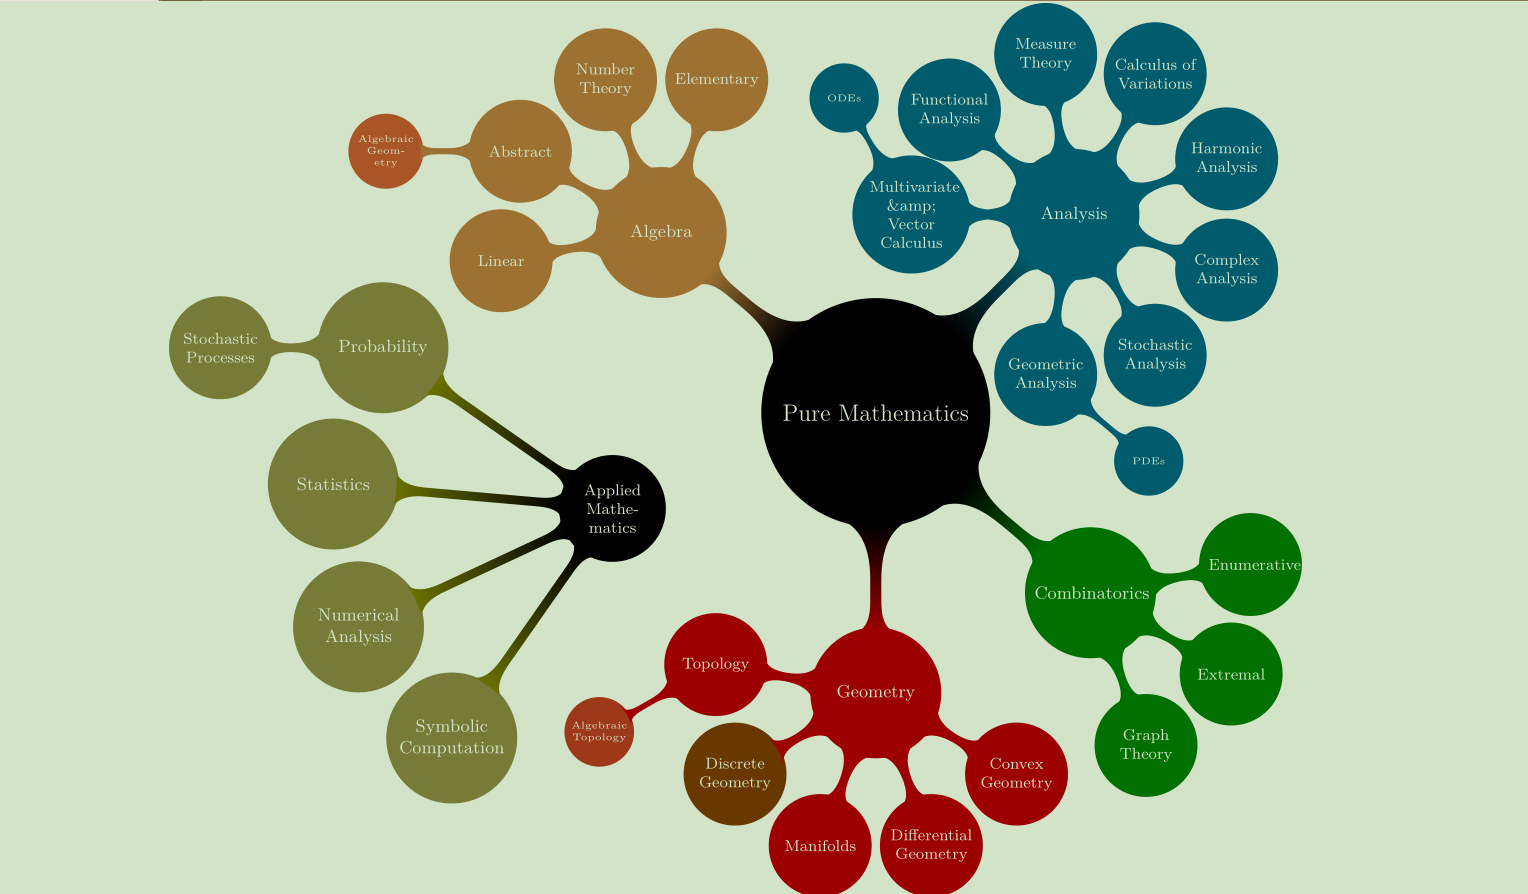
\includegraphics[width=1\textwidth]{112.png}}
\end{figure}
\section{加一个超链接,随你所欲}

\subsection{源代码}
\begin{lstlisting}
	%%%%%%%%%%%%%%%%%%%%%%%%2020.3.26写%%%%%%%%%%%%%%%%%%%%%%%%%%%%%%%%
	这首轻音乐小追真心觉得动听,只要有网,点击一下是可以听的,不妨试试\href{https://t4.kugou.com/song.html?id=70dQS03wjV2
	}{孙子涵的单曲《从夏天开始到夏天结束》\twonotes}
\end{lstlisting}
\subsection{效果展示}
这首轻音乐小追真心觉得动听,只要有网,点击一下是可以听的,不妨试试\href{https://t4.kugou.com/song.html?id=70dQS03wjV2}{孙子涵的单曲《从夏天开始到夏天结束》\twonotes}

\section{运用罗列让表达更具条理}
\subsection{源代码}
\begin{lstlisting}
\textbf{对该笔记使用的一点解释与建议}
\begin{enumerate}
	\item[\ding{172}]\textbf{笔记颜色的使用}
	\begin{itemize}
		\item {\color{red}这是公式,函数等数学符号所使用的颜色}
		\item{\color{gray}这是对函数,公式,概念教材解释所使用的颜色}
		\item \textbf{这是n公式,函数,概念名所使用的颜色}
		\item {\color{green}这是小追自己的补充所使用的颜色}
		\item 表格中的{\color{gray}这种颜色}代表前文已经出现过该公式,函数或概念名
	\end{itemize}
	\item[\ding{173}]\textbf{笔记中思维导图}可以直接点击思维导图下方的超链接可跳转到源思维导图(我自己制作的),源思维导图可能会与笔记中的稍微有点不一样,即我后续改进的。所以相对更加完善些许,如果你想要,可联系我,很乐意发给你的,哈哈
	\item[\ding{174}]\textbf{在笔记中也能听歌}笔记中的\twonotes 标志加入了我所喜欢的音乐,不知合你胃口不,但一定合我胃口,看累了,不妨点击听听试试,看看是否我们有共同喜欢的歌曲。	
\end{enumerate}
\end{lstlisting}
\subsection{效果展示}
\textbf{对该笔记使用的一点解释与建议}
\begin{enumerate}
	\item[\ding{172}]\textbf{笔记颜色的使用}
	\begin{itemize}
		\item {\color{red}这是公式,函数等数学符号所使用的颜色}
		\item{\color{gray}这是对函数,公式,概念教材解释所使用的颜色}
		\item \textbf{这是n公式,函数,概念名所使用的颜色}
		\item {\color{green}这是小追自己的补充所使用的颜色}
		\item 表格中的{\color{gray}这种颜色}代表前文已经出现过该公式,函数或概念名
	\end{itemize}
	\item[\ding{173}]\textbf{笔记中思维导图}可以直接点击思维导图下方的超链接可跳转到源思维导图(我自己制作的),源思维导图可能会与笔记中的稍微有点不一样,即我后续改进的。所以相对更加完善些许,如果你想要,可联系我,很乐意发给你的,哈哈
	\item[\ding{174}]\textbf{在笔记中也能听歌}笔记中的\twonotes 标志加入了我所喜欢的音乐,不知合你胃口不,但一定合我胃口,看累了,不妨点击听听试试,看看是否我们有共同喜欢的歌曲。
\end{enumerate}

\section{用\LaTeX 写数学笔记这些环境还是得了解的}
\subsection{效果展示}
\begin{lemma}{}{}
在齐次线性方程组有非零解的情况下,它有基础解系,并且基础解系所含解的个数等于n-r,这里r表示系数矩阵的秩.(n-r也是自由未知量的个数)
\end{lemma}
\begin{remark}
具体证明过程及讨论可参见高代(北大)P96(有改动)
\end{remark}
\renewcommand{\notename}{小悟}
\begin{note}
\end{note}
\begin{corollary}{和}
fd
\end{corollary}


\begin{example}{和}
fd
\end{example}

\begin{problem}{和}
fd
\end{problem}
\begin{exercise}{和}
fd
\end{exercise}
\begin{conclusion}{和}
fd
\end{conclusion}
\begin{assumption}{和}
fd
\end{assumption}

\begin{property}{和}
\end{property}
\begin{solution}{和}
\end{solution}
%\begin{postulate}{公设3}{e3} 
%\end{postulate}
\begin{proposition}{}{I.48}
A是一实矩阵,则有$r(A^TA)=r(AA^T)=r(A)=r(A^T)$.
\end{proposition}
\begin{definition}{$k$阶子式}{def4}
在$s\times n$矩阵$A$中任意选定$k$行和$k$列$(k\le min\{s,n\})$,位于这些选定的行和列的交点上的$k^2$个元素按原来的次序组成的$k$级行列式,称为$A$的一个$k$阶子式.
\end{definition}
\begin{proof}{}{}
\end{proof}
\begin{theorem}{}{}
	
\end{theorem}
\subsection{源代码}
\begin{lstlisting}
%%%%%%%%%%%%%%%%%%%%%%%%2020.3.26写%%%%%%%%%%%%%%%%%%%%%%%%%%%%%%%%
\begin{lemma}{}{}
在齐次线性方程组有非零解的情况下,它有基础解系,并且基础解系所含解的个数等于n-r,这里r表示系数矩阵的秩.(n-r也是自由未知量的个数)
\end{lemma}
\begin{remark}
具体证明过程及讨论可参见高代(北大)P96(有改动)
\end{remark}
\renewcommand{\notename}{小悟}
\begin{note}
\end{note}
\begin{corollary}{和}
fd
\end{corollary}


\begin{example}{和}
fd
\end{example}

\begin{problem}{和}
fd
\end{problem}
\begin{exercise}{和}
fd
\end{exercise}
\begin{conclusion}{和}
fd
\end{conclusion}
\begin{assumption}{和}
fd
\end{assumption}

\begin{property}{和}
\end{property}
\begin{solution}{和}
\end{solution}
%\begin{postulate}{公设3}{e3} 
%\end{postulate}
\begin{proposition}{}{I.48}
A是一实矩阵,则有$r(A^TA)=r(AA^T)=r(A)=r(A^T)$.
\end{proposition}
\begin{definition}{$k$阶子式}{def4}
在$s\times n$矩阵$A$中任意选定$k$行和$k$列$(k\le min\{s,n\})$,位于这些选定的行和列的交点上的$k^2$个元素按原来的次序组成的$k$级行列式,称为$A$的一个$k$阶子式.
\end{definition}
\begin{proof}{}{}
\end{proof}
\begin{theorem}{}{}

\end{theorem}
\end{lstlisting}

\section{做笔记加背景色一目了然}
\subsection{源代码}
\begin{lstlisting}
%%%%%%%%%%%%%%%%%%%%%%%%2020.3.28写%%%%%%%%%%%%%%%%%%%%%%%%%%%%%%%%
\usepackage{xcolor}
\usepackage[normalem]{ulem} % use normalem to protect \emph
\newcommand\hl{\bgroup\markoverwith
{\textcolor{yellow}{\rule[-.5ex]{2pt}{2.5ex}}}\ULon}
\newcommand\bl{\bgroup\markoverwith
{\textcolor{green}{\rule[-.5ex]{2pt}{2.5ex}}}\ULon}
柯布和道格拉斯研究的是1899年至1922年美国制造业的生产函数。
他们指出,\textbf{制造业的投资}分为\hl{以机器和建筑物为主要形式的固定资本投资和以原料、半成品和仓库里的成品为主要形式的流动资本投资,同时还包括对土地的投资}。\bl{在他们看来,在商品生产中起作用的资本,是不包括流动资本的}。
\end{lstlisting}
\subsection{效果展示}
柯布和道格拉斯研究的是1899年至1922年美国制造业的生产函数。
他们指出,\textbf{制造业的投资}分为\hl{以机器和建筑物为主要形式的固定资本投资和以原料、半成品和仓库里的成品为主要形式的流动资本投资,同时还包括对土地的投资}。\bl{在他们看来,在商品生产中起作用的资本,是不包括流动资本的}。
\section{文章加个背景怎么样}
\subsection{源代码}
\begin{lstlisting}
%%%%%%%%%%%%%%%%%%%%%%%%2020.8.17写%%%%%%%%%%%%%%%%%%%%%%%%%%%%%%%%
\usepackage[all]{background}
%设置背景
\backgroundsetup{scale=1, angle=0, opacity = 1,contents ={
\includegraphics[ keepaspectratio]{0100.jpg}}}
\end{lstlisting}
\subsection{效果展示}
见本文背景
\part{实践成果}

\chapter{ 文章"由一道积分与极限题引发的思考" \footnote{追梦日记2020.数学与逻辑(大学版) \LaTeXe 文二}}
\begin{remark}
	
	一道裴礼文老师只写了提示的题因处处受挫而开始同朋友们探讨,在探讨期间深刻领悟到了变量代换的精髓---区间再现公式,一些较难的积分题的积分技巧和先求导再积分这一方法在本题中的妙用......另外,为了解决一些积分,大致介绍了$\mathrm{Li}_2$函数
	
	I've been discussing a tough question by Pei Liwen (裴礼文) for a long period with my friends\ , whereas few clues given by Li as well as many setbacks I encountered made me frustrated at the commencement\ . During the discussion\ , I deeply comprehended the essence of the interval recurrence formula\ , the skills in evaluating some forms of intractable integrations\ , the methods for integration with some derivation transformations\ .etc\ .Additionally\ ,  in order to evaluate some forms of integrations\ ,  I roughly introduce the dilogarithm function\ . 
\end{remark}


\section{原题}
\begin{prsolbox}
	
	
	\begin{problem}\label{li1}
		证明:
		\[
		\lim_{n\rightarrow\infty}\prod_{i=0}^{n-1}{\left(2+\cos i\frac{\pi}{n}\right)}^{\frac{\pi}{n}}=\left(\frac{\sqrt{3}+2}{2}\right)^{\pi}
		\]
		
		%	\begin{flushright}    
		%		(裴礼文.数学分析中的典型问题与方法.例4.1.3) $^\cite{1}$
		%	\end{flushright} 
	\end{problem}
	
	\begin{flushright}    
		——裴礼文.数学分析中的典型问题与方法.例4.1.3 \cite{1}
	\end{flushright}
\end{prsolbox}
\section{应该会很顺利}
初见此题,易知等式两端取对数,利用定积分的定义即将问题转化为证一个定积分的值,如下:

两端取对数,要证该等式,即证明
$$\frac{\pi}{n}\lim_{n\rightarrow\infty}\sum_{i=0}^{n-1}\ln \left(2+\cos i\frac{\pi}{n}\right)=\pi\ln\frac{\sqrt{3}+2}{2}$$

而等式左端由定积分的定义知,为
$$\frac{\pi}{n}\lim_{n\rightarrow\infty}\sum_{i=0}^{n-1}\ln \left(2+\cos i\frac{\pi}{n}\right)=\int_0^\pi\ln(2+\cos x)\mathrm{d}x$$


即证
$$\int_0^\pi\ln\left(2+\cos x\right)\mathrm{d}x=\pi\ln\frac{\sqrt{3}+2}{2}$$
\section{高大上的死循环}
面对这道积分题,我想到用分部积分法,变量代换和分成子积分。见下面
\subsection{分部积分+变量代换}
\begin{align*}
\int_0^{\pi}{\ln\left(2+\cos x\right)}\mathrm{d}x&=\left. x\ln\left(2+\cos x\right)\right| _{0}^{\pi}+\int_0^{\pi}{\frac{x\sin x}{2+\cos x}}\mathrm{d}x\\
&\xlongequal{t=\pi -x}x\ln\left(2+\cos x\right)\mid_{0}^{\pi}+\int_0^{\pi}{\frac{\left(\pi -t\right)\sin\left(\pi -t\right)}{2+\cos\left(\pi -t\right)}}\mathrm{d}t\\
&=\int_0^{\pi}{\frac{\left(\pi -t\right)\sin t}{2-\cos t}}\mathrm{d}t =\int_0^{\pi}{\frac{\pi\sin t}{2-\cos t}}\mathrm{d}t-\int_0^{\pi}{\frac{t\sin t}{2-\cos t}}\mathrm{d}t\\
&=\pi\ln\left(2-\cos t\right)\mid_{0}^{\pi}-\int_0^{\pi}{\mathrm{d}\left(\ln\left(2-\cos t\right)\right)}\\
&\xlongequal{\textrm{分部积分}}\left.\pi\ln 3-t\ln\left(2-\cos t\right)\right|_{0}^{\pi}+\int_0^{\pi}{\ln}\left(2-\cos t\right)\mathrm{d}t\\
&=\int_0^{\pi}{\ln}\left(2-\cos t\right)\mathrm{d}t
\end{align*}



显然又回到了原地,推出了
\[
\int_0^{\pi}{\ln}\left(2+\cos x\right)\mathrm{d}x=\int_0^{\pi}{\ln}\left(2-\cos t\right)\mathrm{d}t
\]


一个对题目解答毫无帮助的东西
\subsection{分成两个子积分试试}
该思想源于我之前做的一些定积分题如
\[
\int_0^{\frac{\pi}{2}}{f\left(x\right)}\textrm{d}x,\int_0^{\frac{\pi}{4}}{f\left(x\right)}\textrm{d}x
\]
这种类型,经过变量代换后能合并到一起,我们先来看一道之前做过的令我惊奇的定积分题,感受一下这种方法的魅力吧!
\paragraph{一道经典定积分}\footnote{本题在徐森林,金亚东,薛春华.数学分析.第一册[M].北京:清华大学出版社,2007第390-392进行了讨论,除此之外,{\color{orange}还出现在
		(1)浙江大学研究生招生考试《数学分析》试题,2010;
		(2)南京航空航天大学研究生招生考试《数学分析》试题,2005;
		(3)第六十六届美国大学生数学竞赛题,2005;
		(4)第二届北京市大学生数学竞赛题,1990;
		(5)西南交通大学研究生招生考试《数学分析》试题,1987;
		(6)林源渠、方企勤,《数学分析解题指南》,北京大学出版社,2003;
		(7)苏化明,潘杰,唐烁,《高等数学思想方法选讲》,高等教育出版社,2013}\cite{2}\cite{4}}
\begin{problem}\label{li2}
	求\footnote{这里运用\textbf{区间再现公式}解答会更简洁:
		\begin{align*}
		I=&\int_0^{\frac{\pi}{4}}{\ln}\left(1+\tan t\right)\mathrm{d}t=\int_0^{\frac{\pi}{4}}{\ln}\left[1+\tan\left(\frac{\pi}{4}-t\right)\right]\mathrm{d}t=\int_0^{\frac{\pi}{4}}{\ln}\left(\frac{2}{1+\tan t}\right)\mathrm{d}t\\
		=&\int_0^{\frac{\pi}{4}}{\left[\ln 2-\ln\left(1+\tan t\right)\right]}\mathrm{d}t=\frac{\ln 2}{4}\pi -I\Longrightarrow I=\frac{\pi\ln 2}{8}
		\end{align*}}
	$y=\int_0^1 \frac{\ln (1+x)}{1+x^2}\mathrm{d}x$ 
\end{problem}
\begin{solution}
	\textbf{法一}(三角换元)(例\ref{li2}): 
	
	令$x=\tan t,\mathrm{d}x=\frac{1}{\cos^2t}\mathrm{d}t,t\in\left(0,\frac{\pi}{4}\right)$,即
	\begin{align*}
	y&=\int _0^\frac{\pi}{4}\ln (1+\tan t)\mathrm{d}t=\int_0^{\frac{\pi}{4}}{\ln}\left(\frac{\sqrt{2}\sin\left(t+\frac{\pi}{4}\right)}{\cos t}\right)\mathrm{d}t\\
	&=\int_0^{\frac{\pi}{4}}{\ln}\sqrt{2}\mathrm{d}t+\int_0^{\frac{\pi}{4}}{\ln}\sin\left(t+\frac{\pi}{4}\right)\mathrm{d}t-\int_0^{\frac{\pi}{4}}{\ln}\cos t\mathrm{d}t
	\end{align*}
	
	令$u=\frac{\pi}{4}-t,u\in\left(0,\frac{\pi}{4}\right)$,即
	\[
	\int_0^{\frac{\pi}{4}}{\ln}\sin\left(t+\frac{\pi}{4}\right)\mathrm{d}t=\int_0^{\frac{\pi}{4}}{\ln}\cos u\mathrm{d}u
	\]
	则
	\[y=\int_0^\frac{\pi}{4}\ln \sqrt{2}\mathrm{d}t=\ln \sqrt {2}t\rvert_0^\frac{\pi}{4}=\frac{\ln 2}{8}\pi\]
	
	本题经过变量代换后得到与原式相同的式子合并及求出,而要讨论的这道题行不通吗?
	\[
	\int_0^\pi \ln (2+\cos x)\mathrm{d}x=\int_0^\frac{\pi}{2} \ln (2+\cos x)\mathrm{d}x+\int_\frac{\pi}{2}^\pi \ln (2+\cos x)\mathrm{d}x\]
	其中
	\[
	\int_{\frac{\pi}{2}}^{\pi}{\ln}\left(2+\cos x\right)\mathrm{d}x\xlongequal{t=\pi -x}\int_0^{\frac{\pi}{2}}{\ln}\left(2-\cos t\right)\mathrm{d}t
	\]
	即
	\[ \text{原式}= \int_0^\frac{\pi}{2}\ln (2+\cos x)\mathrm{d}x+\int_0^\frac{\pi}{2}\ln (2-\cos t)\mathrm{d}t\]
\end{solution}
\subsection{再进行变量代换试试}
其中\[
\int_0^\frac{\pi}{2}\ln (2+\cos x)\mathrm{d}x\xRightarrow{t=\frac{\pi}{2}-x}\int_0^\frac{\pi}{2}\ln (2+\sin t)\mathrm{d}t\]

其中\[
\int_0^\frac{\pi}{2}\ln (2-\cos t)\mathrm{d}t\xRightarrow{x=\frac{\pi}{2}-t}\int_0^\frac{\pi}{2}\ln (2-\sin x)\mathrm{d}x\]
\[\text{即原式}=\int_0^\frac{\pi}{2}\ln (2+\sin t)\mathrm{d}t+\int_0^\frac{\pi}{2}\ln (2-\sin x)\mathrm{d}x\]


易看出即使进行分部积分也不会得到想要的结果,只会不断循环,花了很多时间推出了下面这些等式,对解答毫无帮助的东西,心塞.
\begin{itemize}
	\item$\int_0^\frac{\pi}{2}\ln (2+\sin t)\mathrm{d}t=\int_0^\frac{\pi}{2}\ln (2+\cos t)\mathrm{d}t$
	\item$\int_0^\frac{\pi}{2}\ln (2-\cos t)\mathrm{d}t=\int_0^\frac{\pi}{2}\ln (2-\sin t)\mathrm{d}t$
\end{itemize}
\section{光明来临?}
一位学长突然来信说,他解出来了,用了区间再现公式,我内心十分激动,区间再现公式?我首先看的就是他分享给我的有关区间再现公式文档\cite{3}。
\begin{conclusion}[区间再现公式\footnote{证明它极其容易,即直接作变量代换,令$x=a+b-t$易证得。}] 
	$$\int_a^bf(x)\mathrm{d}x=\int_a^b f(a+b-x)\mathrm{d}x$$
\end{conclusion}
看完全文后,我感到十分欣喜,公式名之前没听过,但所列举的题目有些是我曾经感到不解的,如证明以下等式:
\begin{problem}
	$\int_0^\frac{\pi}{2}\frac{\sin x}{\sin x+\cos x}\mathrm{d}x=\int_0^\frac{\pi}{2}\frac{\cos x}{\sin x+\cos x}\mathrm{d}x=\frac{\pi}{4}$
\end{problem}
\begin{problem}$\int_0^\pi\frac{x\sin x}{1+\cos ^2x} \mathrm{d}x=\frac{\pi}{2}\int_0^\pi\frac{\sin x}{1+\cos ^2x}\mathrm{d}x=\pi\int_0^\frac{\pi}{2}\frac{\sin x}{1+\cos ^2x}=\frac{\pi ^2}{4} $
\end{problem}
\begin{problem}$\int_0^1x^m(1-x)^n \mathrm{d}x=\int_0^1 x^n(1-x)^m\mathrm{d}x$
\end{problem}
\begin{problem}
	$\int_0^\frac{\pi}{2}f(\sin x)\mathrm{d}x=\int_0^\frac{\pi}{2}f(\cos x)\mathrm{d}x=\frac{1}{2}\int_0^\pi f(\sin x)\mathrm{d}x
	$	
\end{problem}
这些题老师与参考解析都会生硬的告诉你做变量代换,而现在用上这个公式后用大彻大悟这个词来形容也不为过了,欣喜之余,再回过头来看学长的解答,可是发现计算出了小错误,自己用这个公式再做了一遍,最后还是进入了死循环,并发现我之前的计算过程中其实也在不经意间用了区间再现公式。看来白欢喜了一场,但至少系统的学到了这种方法,也很满足了!
\section{该题的终结者?}
在自己思考的同时,我把题目分享给了更多人,希望之后有大佬来指点。有幸的是,一天后,惠民学长在傍晚时分给了我一个简洁的解答。如下:
\begin{solution}\textbf{法一:}(例\ref{li1})令
	\begin{align}
	I\left(\theta\right)=\int_0^{\pi}{\ln}\left(1+\theta\cos x\right)\mathrm{d}x,\quad \theta\in\left(-1,1\right)\label{1.1}
	\end{align}
	{\color{gray}\begin{equation} \begin{aligned}
		I'\left(\theta\right)&=\int_0^{\pi}{\frac{\partial\ln\left(1+\theta\cos x\right)}{\partial\theta}}\mathrm{d}x=\int_0^\pi \frac{\cos x}{1+\theta \cos x}\mathrm{d}x=\frac{\pi}{\theta}-\frac{1}{\theta}\int_0^\pi\frac{1}{1+\theta \cos x}\mathrm{d}x\\
		&\xlongequal{t=\tan (\frac{x}{2})}\frac{\pi}{\theta}-\frac{1}{\theta}\int_0^{+\infty} \frac{2}{(1-\theta)+( 1+\theta)t^2}\mathrm{d}t\\
		&\left. =\frac{\pi}{\theta}-\frac{2}{\theta\left(1+\theta\right)}\sqrt{\frac{1+\theta}{1-\theta}}\arctan\left(\sqrt{\frac{1+\theta}{1-\theta}}t\right)\right|_{0}^{+\infty}\\
		&=\frac{\pi}{\theta}-\frac{\pi}{\theta\sqrt{1-\theta^2}}
		\end{aligned} \end{equation}}
	查积分表得:
	\begin{align*}
	I(\theta)=\int_0^\theta\left(\frac{\pi}{\theta}-\frac{\pi}{\theta\sqrt{1-\theta^2}}\right)\mathrm{d}\theta +I(0)=\pi \ln \frac{1+\sqrt{1-\theta^2}}{2}
	\end{align*}
	所以
	\[\int_0^\pi\ln \left(2+\cos x\right)\mathrm{d}x=\int_0^\pi\left(\ln \left(1+\frac{1}{2}\cos x\right)+\ln 2\right)\mathrm{d}x\\
	=I\left(\frac{1}{2}\right)+\pi\ln 2
	=\pi \ln \left(\frac{2+\sqrt{3}}{2}\right)\]
\end{solution}
\begin{note}
	\begin{itemize}
		\item[*]该法中(2)用到了含参量积分求导公式
		\begin{conclusion}[含参量积分求导公式]\cite{6}
			若 $c(x),d(x)$为定义在$[a,b]$上其值含于$[p,q]$内的可微函数,则$F(x)=\int_{c(x)}^{d(x)}f(x,y)\mathrm{d}y$
			在$[a,b]$上可微,且
			$$F'(x)=\int_{c(x)}^{d(x)}f_x(x,y)\mathrm{d}y+f(x,d(x))\mathrm{d}'(x)-f(x,c(x))c'(x)$$
		\end{conclusion}
		
	\end{itemize}
\end{note}

看了该解答后有种妙不可言的感觉,先求通式,通式用先求导再积分得到,再将所求的问题通过取数值带入即可,但同时我脑海里也出现了如下疑问:
\begin{itemize}
	\item 为什么是求通式$I(\theta)=\int_0^\pi\ln (1+\theta \cos x)\mathrm{d}x$?而不是求
	
	$I(\theta)=\int_0^\pi\ln (\theta+\cos x)\mathrm{d}x$    
	\item 先求导,再积分似曾相识,在这里为什么行得通?
	\item 积分表?如果是考试呢?即它的完整过程是怎样的?
	\item 能否进行推广,如求$\int_0^\pi\ln(1+\theta\cos x)\mathrm{d}\theta$,$\int_a^b\ln (1+\theta f(x))\mathrm{d}\theta$等
\end{itemize}
\subsection{都可以}
求$I(\theta)=\int_0^\pi\ln (\theta+\cos x)\mathrm{d}\theta$也是可以的,只是 $\theta$ 的范围需要变化,感兴趣的朋友不妨试试!
\subsection{记忆尤在}
我们知道定积分
$\int_a^b f(x)\mathrm{d}x$ ($a,b$为常数;$f(x)$为一元函数)是一个常数,而当$f(x)$为二元函数时,即如$I(\theta)=\int_0^\pi f(\theta,x)\mathrm{d}x$求出来后是一个关于 $\theta$的一元函数,当原函数不好求时,进行求导,如求
$I(\theta)=\int_0^\pi \ln (1+\theta \cos x)\mathrm{d}x$时,对$\theta$求偏导,得
\[
I'\left(\theta\right)=\int_0^{\pi}{\frac{\cos x}{1+\theta\cos x}}\mathrm{d}x
\]

易看出该定积分是我们所熟悉的,用万能公式即可求出,化为关于$\theta$的函数后再求$\theta$的不定积分即得出,重点是$\theta$ 的积分变为易可求的,笔者认为用了化简为繁的思想。
先求导再积分的方法,之前在求  $\arctan x$ 的级数时应用到了,即先对它求导变为$\frac{1}{1+x^2}$再对该函数进行泰勒展开,之后再积分回去即求得.
当然,那道\textbf{经典定积分例 \ref{li2} }\cite{4} 也可运用此法
\begin{proof}
	\textbf{法二:}(例 \ref{li2} ) 令
	\[y
	(\alpha)=\int_0^\alpha\frac{\ln(1+\alpha x)}{1+x^2}\mathrm{d}x\]
	则$y=y(1),y(0)=0$,且$y(\alpha)$满足对$\alpha$ 的求导条件,于是
	\[
	y'\left(\alpha\right)=\frac{\ln\left(1+\alpha^2\right)}{1+\alpha^2}+\int_0^{\alpha}{\frac{x}{\left(1+x^2\right)\left(1+\alpha x\right)}}\mathrm{d}x=\frac{\ln\left(1+\alpha^2\right)}{2\left(1+\alpha^2\right)}+\frac{\alpha\arctan y}{1+y^2}
	\]
	上式两端从0到$y$积分,得
	\[
	y\left(\alpha\right)=\frac{1}{2}\left[\int_0^{\alpha}{\ln}\left(1+t^2\right)\mathrm{d}\left(\arctan t\right)+\int_0^{\alpha}{\arctan}\,\,t\mathrm{d}\left(\ln\left(1+t^2\right)\right)\right]=\frac{1}{2}\ln\left(1+\alpha^2\right)\arctan\alpha 
	\]
	所以
	\[y=y(1)=\frac{1}{2}\ln(1+1) \arctan 1=\frac{\pi}{8}\ln 2\]
	
	\textbf{法三:}(例\ref{li2})令
	\[y
	(\alpha)=\int_0^1\frac{\ln(1+\alpha x)}{1+x^2}\mathrm{d}x\]
	则$y=y(1),y(0)=0$,且$y(\alpha)$满足对$\alpha$ 的求导条件,于是
	\[y'(\alpha)=\int_0^1\frac{x}{(1+x^2)(1+\alpha x)}\mathrm{d}x\]
	其中定积分中的被积函数可以拆分为
	\[\frac{x}{(x^2+1)(\alpha x+1)}=\frac{a}{a^2+1}\frac{1}{x^2+1}+\frac{1}{a^2+1}\frac{x}{x^2+1}-\frac{a}{a^2+1}\frac{1}{\alpha x+1}\]
	所以积分可得
	\[
	y'\left(\alpha\right)=\frac{1}{1+\alpha^2}\left[\frac{1}{2}\ln 2+\frac{\pi}{4}\alpha -\ln\left(1+\alpha\right)\right]
	\]
	上式对$\alpha$从0到1积分,得
	\[
	\left. y\left(1\right)-y\left(0\right)=\left[\frac{1}{2}\ln 2\cdot\arctan\alpha +\frac{\pi}{8}\ln\left(1+\alpha^2\right)\right]\right|_{0}^{1}=\frac{\pi}{4}\ln 2-y\left(1\right)
	\]
	所以\[y=y(1)=\frac{\pi}{8}\ln2\]
	
\end{proof}
\subsection{完整的解答(例\ref{li1})}
现在,让我们完整的表达下\\
\begin{proof}两端取对数,要证该不等式,即证 
	\[
	\frac{\pi}{n}\lim_{n\rightarrow\infty}\sum_{i=0}^{n-1}\ln \left(2+\cos i\frac{\pi}{n}\right)=\pi\ln\frac{\sqrt{3}+2}{2}\]
	由定积分的定义得
	\[\frac{\pi}{n}\lim _{n\to \infty}\sum_{i=0}^{n-1}\ln \left(2+\cos i\frac{\pi}{n}\right)
	=\int_0^\pi\ln (2+\cos x)\mathrm{d}x\]
	即证
	\[\int_0^\pi\ln (2+\cos x)\mathrm{d}x
	=\pi \ln \left(\frac{\sqrt{3}+2}{2}\right)\]
	先令
	\[
	I\left(\theta\right)=\int_0^{\pi}{\ln}\left(1+\theta\cos x\right)\mathrm{d}x,\qquad\theta\in\left[-1,1\right]
	\]
	\begin{align*}
	I'\left(\theta\right)&=\int_0^{\pi}{\frac{\cos x}{1+\theta\cos x}}\mathrm{d}x=\frac{\pi}{\theta}-\frac{1}{\theta}\int_0^{\pi}{\frac{1}{1+\theta\cos x}}\mathrm{d}x\xlongequal{t=\tan\frac{x}{2}}\frac{\pi}{\theta}-\frac{1}{\theta}\int_0^{+\infty}{\frac{2}{\left(1-\theta\right)+\left(1+\theta\right)t^2}}\mathrm{d}t\\
	&\left. =\frac{\pi}{\theta}-\frac{2}{\theta\left(1+\theta\right)}\sqrt{\frac{1+\theta}{1-\theta}}\arctan\left(\sqrt{\frac{1+\theta}{1-\theta}}t\right)\right|_{0}^{+\infty}=\frac{\pi}{\theta}-\frac{\pi}{\theta\sqrt{1-\theta^2}}
	\end{align*}
	{\color{gray}{因此
			\begin{align*}
			I\left(\theta\right)&=\int{\left(\frac{\pi}{\theta}-\frac{1}{\theta}\frac{\pi}{\sqrt{1-\theta^2}}\right)}\textrm{d}\theta =\pi\ln\theta -\pi\int{\frac{1}{\theta\sqrt{1-\theta^2}}}\textrm{d}\theta\xlongequal{\theta =\sin x}\pi\ln\theta -\pi\int{\frac{1}{\sin x}}\textrm{d}x\\
			&=\pi\ln\theta +\pi\ln\left(\cot x+\csc x\right)+C=\pi\ln\theta +\pi\ln\left(\frac{1+\cos x}{\sin x}\right)+C\\
			& =\pi\left(\ln\theta +\ln\frac{1+\sqrt{1-\theta^2}}{\theta}\right)+C=\pi\ln\left(1+\sqrt{1-\theta^2}\right)+C
			\end{align*}
			由于$I(0)=0$,即$C=-\ln 2$,即证.}}
	
	对于
	\begin{align*}
	\int{\frac{1}{\theta\sqrt{1-\theta^2}}}\mathrm{d}\theta&\xlongequal{\theta =\sin r}\int{\frac{1}{\sin r\cos r}}\cos r\mathrm{d}r=\int{\frac{1}{\sin r}}\mathrm{d}r\\
	&\left.\left. =\int{\frac{\csc r\left(\csc r-\cot r\right)}{\csc r-\cot r}}\mathrm{d}r=\ln\right|\csc r-\cot r\right|+C
	\end{align*}
	构造直角三角形,易知有
	$$\csc r=\frac{1}{\theta},\quad\cot r=\frac{\sqrt{1-\theta^2}}{\theta}$$
	即
	\[
	\left.\left.\int{\frac{1}{\theta\sqrt{1-\theta^2}}}\mathrm{d}\theta =\ln\right|\frac{1}{\theta}-\frac{\sqrt{1-\theta^2}}{\theta}\right|+C=\ln\left(\frac{\theta}{1+\sqrt{1-\theta^2}}\right)+C
	\]
	因此
	\[
	\int{I}'\left(\theta\right)\mathrm{d}\theta =\pi\ln\theta -\pi\ln\left(\frac{\theta}{1+\sqrt{1-\theta^2}}\right)+C=\pi\ln\left(1+\sqrt{1-\theta^2}\right)+C
	\]
	\[
	\Rightarrow I\left(\theta\right)=\int_0^{\theta}{I}'\left(\theta\right)\mathrm{d}\theta =\left. \pi\ln\left(1+\sqrt{1-\theta^2}\right)\right| _{0}^{\theta}+I\left(0\right)
	\]
	\[
	\int_0^{\pi}{\ln}\left(2+\cos x\right)\mathrm{d}x=\int_0^{\pi}{\ln}\left(1+\frac{1}{2}\cos x\right)\mathrm{d}x+\int_0^{\pi}{\ln}2\mathrm{d}x=I\left(\frac{1}{2}\right)+\pi\ln 2=\pi\ln\left(1+\frac{\sqrt{3}}{2}\right)
	\]
\end{proof}
\subsection{推广的辛酸}
试求 \[
I\left(\theta\right)=\int_0^{\pi}{\ln}\left(1+\theta\sin x\right)\mathrm{d}x
\]的路,我以为换汤不换药,应该不难,没想到换了一个碗!看下面的心酸过程

\begin{problem} 
	求$$I(\theta)=\int_0^\pi \ln (1+\theta\sin x)\mathrm{d}x\qquad\theta\in(-1,1)$$\end{problem}
\begin{solution}
	含参处理
	\begin{align*}
	I'\left(\theta\right)&=\int_0^{\pi}{\frac{\sin x}{1+\theta\sin x}}\mathrm{d}x=\int_0^{\pi}{\frac{1}{\theta}}\mathrm{d}x-\frac{1}{\theta}\int_0^{\pi}{\frac{1}{1+\theta\sin x}}\mathrm{d}x\xlongequal{t=\tan\frac{x}{2}}\int_0^{\pi}{\frac{1}{\theta}}\mathrm{d}x-\frac{1}{\theta}\int_0^{+\infty}{\frac{2}{t^2+2\theta t+1}}\mathrm{d}t\\
	&=\frac{\pi}{\theta}-\frac{2}{\theta}\int_0^{+\infty}{\frac{1}{\left(t+\theta\right)^2+\left(\sqrt{1-\theta^2}\right)^2}}\mathrm{d}t=\frac{\pi}{\theta}-\left. \frac{2}{\theta}\left(\frac{1}{\sqrt{1-\theta^2}}\arctan\left(\frac{t+\theta}{\sqrt{1-\theta^2}}\right)\right)\right| _{0}^{+\infty}\\
	&=\frac{\pi}{\theta}-\frac{\pi}{\theta\sqrt{1-\theta^2}}+\frac{2}{\theta\sqrt{1-\theta^2}}\arctan\left(\frac{\theta}{\sqrt{1-\theta^2}}\right)
	\end{align*}
	下面需要求
	\[
	\int{I}'\left(\theta\right)\mathrm{d}\theta =\int{\left(\frac{\pi}{\theta}-\frac{\pi}{\theta\sqrt{1-\theta^2}}\right)}\mathrm{d}\theta +\int{\frac{2}{\theta\sqrt{1-\theta^2}}}\arctan\left(\frac{\theta}{\sqrt{1-\theta^2}}\right)\mathrm{d}\theta 
	\]
	可以很快发现
	\[
	\int{\left(\frac{\pi}{\theta}-\frac{\pi}{\theta\sqrt{1-\theta^2}}\right)}\mathrm{d}\theta 
	\]
	是在求$\int_0^\pi \ln (1+\theta\cos x)\mathrm{d}x$时所需求的不定积分,而求
	$$\int\frac{2}{\theta\sqrt{1-\theta^2}}\arctan\left(\frac{\theta}{\sqrt{1-\theta^2}}\right)\mathrm{d}\theta$$
	
	不简单,下面是学友$2^\aleph$对本题的解答
\end{solution}
\subsubsection{真不简单(dilogarithm函数)}
\begin{problem}
	求
	\[
	\int{\frac{2}{\theta\sqrt{1-\theta^2}}}\arctan\left(\frac{\theta}{\sqrt{1-\theta^2}}\right)\mathrm{d}\theta 
	\]
\end{problem}
\begin{solution}
	令$\theta =\sin x, x\in\left(-\frac{\pi}{2},0\right)\cup\left(0,\frac{\pi}{2}\right)$,则有
	\[
	\int{\frac{2}{\theta\sqrt{1-\theta^2}}}\arctan\left(\frac{\theta}{\sqrt{1-\theta^2}}\right)\mathrm{d}\theta =\int{\frac{2x}{\sin x\cos x}}\mathrm{d}\sin x=\int{\frac{2x}{\sin x}}\mathrm{d}x
	\]
	由Euler公式$\sin x=\frac{\mathrm{e}^{\mathrm{i}x}-\mathrm{e}^{-\mathrm {i}x}}{2\mathrm {i}}$得
	{\color{orange}\begin{align*}
		\int\frac{2x}{\sin x}\mathrm{d}x&=\int \frac{2\mathrm {i} \cdot 2x}{\mathrm{e}^{\mathrm {i}x}-\mathrm{e}^{-\mathrm {i}x}}\mathrm{d}x=4\int \frac{\mathrm {i}x}{\mathrm{e}^{\mathrm {i}x}-\mathrm{e}^{-\mathrm {i}x}}\mathrm{d}x\xlongequal{u=\mathrm {i}x}
		4\int \frac{-u\mathrm{e}^u\mathrm {i}}{\mathrm{e}^{2u}-1}\mathrm{d}u\\
		&\xlongequal{v=\mathrm{e}^u}-4\mathrm {i}\int \frac{\ln v}{v^2-1}\mathrm{d}v=2\mathrm {i}\left[\int \frac{\ln v}{v+1}\mathrm{d}v-\int \frac{\ln v }{v-1}\mathrm{d}v\right]\\
		&\xlongequal{\text{分部积分得}}
		2\mathrm {i}\left[\ln v(\ln (v+1)+\ln(v-1))-\int \frac{\ln (v+1)}{v}\mathrm{d}v+\int \frac{\ln (v-1)}{v} \mathrm{d}v\right]
		\end{align*}}
	引入\footnote{$\mathrm{Li}_2(x)=\frac{x}{1}+\frac{x^2}{2^2}+\frac{x^3}{3^2}+\cdots=\int_0^x\frac{-\ln (1-x)}{x}\mathrm{d}x$}$\mathrm{Li}_2(x)=\int_0^x -\frac{\ln (1-x)}{x}\mathrm{d}x,$
	%%%%%%%%%%%%%%%%%%%%%%%%%%%%%%%%%%%%%%%
	先证引理\footnote{限于篇幅,关于$\mathrm{Li}_2(x)$的更多内容可参见\cite{5}	
		$\mathrm{Li}_2(1)=\frac{1}{1}+\frac{1}{2^2}+\frac{1}{3^2}+\cdots =\frac{\pi ^2}{6}$,\quad  $\mathrm{li}(x)=\int \frac{1}{\ln x}\mathrm{d}x$}:$$\mathrm{Li}_2(x)+\mathrm{Li}_2(1-x)=\frac{\pi^2}{6}-\ln x\ln (1-x)$$
	%%%%%%%%%%%%%%%%%%%%%%%%%%%%%%%%%%%%%%%%%%%
	\begin{proof}
		\begin{align*}
		\mathrm{Li}_2(x)&=\int_0^x\frac{-\ln(1-x)}{x}\mathrm{d}x=\int _0^x-\ln (1-x)d\ln x\\
		&\xlongequal{\text{分部积分}}-\ln (1-\pi)\ln x+\int_0^x\frac{\ln x}{x-1}\mathrm{d}x\\
		&=-\ln x\ln (1-x)+\mathrm{Li}_2(1)-\mathrm{Li}_2(1-x)\\
		\end{align*}
		\[
		\Longrightarrow\mathrm{Li}_2\left(x\right)+\mathrm{Li}_2\left(1-x\right)=-\ln x\ln\left(1-x\right)+\frac{\pi^2}{6}
		\]
		代入化简得
		\begin{align*}
		\text{原式}&=2\mathrm{i}\left[\ln \left(\mathrm{e}^{\mathrm{i}x}\right)\ln 
		\left(\mathrm{e}^{\mathrm{i}x}+1\right)-\ln \mathrm{e}^{\mathrm{i}x}\ln\left(\mathrm{e}^{\mathrm{i}x}-1\right)+\mathrm{Li}_2\left(-\mathrm{e}^{\mathrm{i}x}\right)-\mathrm{Li}_2\left(1-\mathrm{e}^{\mathrm{i}x}\right)\right]+C\\
		&=2\mathrm{i}\left[\ln \left(\mathrm{e}^{\mathrm{i}x}\right)\ln \left(\mathrm{e}^{\mathrm{i}x}+1\right)-\ln \left(\mathrm{e}^{\mathrm{i}x}\right)\ln\left(\mathrm{e}^{\mathrm{i}x}-1\right)+\frac{\pi^2}{6}-\ln \left(\mathrm{e}^{\mathrm{i}x}\right)\ln \left(1-\mathrm{e}^{\mathrm{i}x}\right)\right]+C\\
		\end{align*}
		注意到$x\in\left(-\frac{\pi}{2},0\right)\cup\left(0,\frac{\pi}{2}\right),\quad\ln (z)=\ln|z|+\mathrm{i}arg(z),$
		\begin{align*}
		\text{上式}=2\mathrm{i}\left[\frac{\pi^2}{6}-\mathrm{i}x\ln(\mathrm{e}^{\mathrm{i}x}+1)+\mathrm{i}x\ln(\mathrm{e}^{\mathrm{i}x}-1)+\mathrm{i}\ln\left(1-\mathrm{e}^{\mathrm{i}x}\right)\right]+C\\
		=\frac{\mathrm{i}\pi^2}{3}+2x\ln\left(\mathrm{e}^{ix}+1\right)-2x\ln\left(\mathrm{e}^{\mathrm{i}x}-1\right)-2x\ln\left(1-\mathrm{e}^{\mathrm{i}x}\right)+C
		\end{align*}
		上式为实值函数,故取实数部分即可
		\begin{align*}
		\text{上式}&=2x\ln\left|1+\mathrm{e}^{\mathrm{i}x}\right|-4x\ln\left|1-\mathrm{e}^{\mathrm{i}x}\right|+c\\
		&=x\ln\left|\left(1+\cos x\right)^2+\left(\sin x\right)^2\right|-2x\ln\left|\left(1-\cos x\right)^2+(\sin x)^2\right|+C\\
		&=x\ln \left(\frac{2+2\cos x}{(2-2\cos x)^2}\right)+C
		=\arcsin \theta\ln \left(\frac{2+2\sqrt{1-\theta^2}}{\left(2-2\sqrt{1-\theta^2}\right)^2}\right)+C
		\end{align*}
		所以
		{\color{gray}\[
			I_1\left(\theta\right)=\int{\ln}\left(1+\theta\sin x\right)\mathrm{d}x=\arcsin\theta\ln\left(\frac{2+2\sqrt{1-\theta^2}}{\left(2-2\sqrt{1-\theta^2}\right)^2}\right)+\pi\ln\left(1+\sqrt{1-\theta^2}\right)+c
			\]}
		又$I(0)=0$,则有
		\[
		I\left(\theta\right)=\int_0^{\pi}{\ln}\left(1+\theta\sin x\right)\mathrm{d}x=\arcsin\theta\ln\left(\frac{2+2\sqrt{1-\theta^2}}{\left(2-2\sqrt{1-\theta^2}\right)^2}\right)+\pi\ln\left(1+\sqrt{1-\theta^2}\right)-\pi\ln 2
		\]
		
		显然比求
		$ \int_0^\pi\ln (2+\cos x)\mathrm{d}x$
		还难很多。而求
		\[
		I\left(\theta\right)=\int_c^d{\ln}\left(1+\theta f\left(x\right)\right)\textrm{d}x
		\]
		用这种方法的思路还是比较系统的
	\end{proof}
\end{solution}
\begin{problem} 
	求\[
	I\left(\theta\right)=\int_c^d{\ln}\left(1+\theta f\left(x\right)\right)\mathrm{d}x
	\]
	
\end{problem}
\begin{solution}
	显然
	\[
	I'\left(\theta\right)=\int_c^d{\frac{f\left(x\right)}{1+\theta f\left(x\right)}}\mathrm{d}x=\int_c^d{\frac{1}{\theta}}\mathrm{d}x-\frac{1}{\theta}\int_c^d{\frac{1}{1+\theta f\left(x\right)}}\mathrm{d}x=\frac{1}{\theta}\left[\left(d-c\right)-\int_c^d{\frac{1}{1+\theta f\left(x\right)}}\right]\mathrm{d}x
	\]
	令$F(x)$为$\frac{1}{1+\theta f(x)}$的原函数,$F(x)$中含有$\theta$
	\[
	I'\left(\theta\right)=\frac{1}{\theta}\left[\left(d-c\right)-F\left(d\right)+F\left(c\right)\right]
	\]
	\[
	\Rightarrow\int{I}'\left(\theta\right)\mathrm{d}\theta =\left(d-c\right)\ln\theta -\int{\frac{1}{\theta}}\left[F\left(d\right)-F\left(c\right)\right]\mathrm{d}\theta 
	\]
	令$G(\theta)$为$\frac{F(d)-F(c)}{\theta}$的原函数,当$(d-c)\ln \theta$与$G(\theta)$能够合并时,令合并后为$H(\theta)$
	
	(若不能合并,则该法行不通)
	
	得\[
	I\left(\theta\right)=H\left(\theta\right)\mid_{0}^{\theta}+I\left(0\right)
	\]
	经过与朋友讨论后发现该法降低了可求$I(\theta)$的概率,如下
	\begin{itemize}	
		\item$F(x)$需能求得出,即$\int \frac{1}{1+\theta f(x)}\mathrm{d}x$可积
		\item$G(\theta)$需能求得出,即$\int\frac{F(d)-F(c)}{\theta}\mathrm{d}\theta$可积
		\item$(d-c)\ln\theta$与$G(\theta)$要能够合并为一整体,不然$\ln\theta|_0^\theta$这是没有意义的
	\end{itemize}
	
	{\color{gray}这三道关卡必须全部通过,缺一不可,才能求出,并且令人不快的是,很简单的函数如
		$f(x)$为常数或$x$,相比用分部积分法困难多了,不妨试试,当然感兴趣的朋友也可探究下 $f(x)$为哪些函数时只能用这种方法求得出或求不出等等.}
\end{solution}
\section{裴老师的密码?}	
裴礼文老师对于这道题只是简单的提了如下一句话:

{\color{gray}提示:先取对数,积分可用分部积分法及变量替换 $\pi -x=t$  求解。(博士论坛对此题有详细的讨论)\cite{1}}

是老师觉得这道题太简单了?为什么用老师提供的这一思路似乎无法达到预料的效果?老师出这本书时,是从1988年的笔者的话,到1993年五月第一版,2006年四月第二版,最短跨度也已经有近14年了,说这道题在博士数学论坛上面有详细讨论,去寻找不是犹如大海捞针么?这道题能否用老师提示的方法做出来,或者是否有更好的解法,期待你的解答\footnote{小追:
	
	QQ邮箱:hzjxkqh@qq.com
	
	QQ:2357239474
	
}!
\section{再续前缘}
的确,生活处处充满惊喜,探究这道题,一路走来,步步深入,收获颇多,本来应该即将完结的!而前方等待我的却还有更大的惊喜,更多的收获!今天(2.7)有幸同八一学长讨论,发现还有更多的秘密,可见下面解答见\href{https://mp.weixin.qq.com/s/554E8awja77ekIIGNEK9vw}{习题讲义之问题求解(练习17.3)}……
\subsection{另一种神奇的解法}

\textbf{法二:}\footnote{在数学论坛Mathematics Stack Exchange上用这种方法(Gauss MVT)详细的讨论了一道与本题相似的积分题,感兴趣的可以复制以下链接:
	\url{https://math.stackexchange.com/questions/354795/evaluate-int-0-pi-ln-left-sin-theta-right-d-theta}
}(例\ref{li1})
\begin{solution}
	显然
	\begin{align}
	\text{原式}= \int_0^\pi \ln(2+\cos x)\mathrm{d}x=\frac{1}{2}\int_0^{2\pi}\ln (2+\cos x)\mathrm{d}x
	\end{align}
	由于
	\begin{align}
	4\pi\ln \left(\sqrt{3}+3\right)&=\int_0^{2\pi}\left[\ln\left(\sqrt{3}+2+\mathrm{e}^{\mathrm{i}x}\right)+\ln \left(\sqrt{3}+2+\mathrm{e}^{-\mathrm{i}x}\right) \right] \mathrm{d}x\\&
	=\int_0^{2\pi}\ln\left[\left(\sqrt{3}+2\right)^2+2\left(\sqrt{3}+2\right)\cos x+1\right]\mathrm{d}x\\&
	=\int_0^{2\pi}\ln\left[4\left(2+\sqrt{3}\right)+2\left(2+\sqrt{3}\right)\cos x\right]\mathrm{d}x \notag \\
	&=\int_0^{2\pi}\ln\left(2\left(2+\sqrt{3}\right)\right)\mathrm{d}x+\int_0^{2\pi}\ln (2+\cos )\mathrm{d}x\notag 
	\end{align}
	即
	\[
	\int_0^{2\pi}{\ln}\left(2+\cos x\right)\mathrm{d}x=2\pi\ln\left(\frac{\left(2+\sqrt{3}\right)^2}{2\left(2+\sqrt{3}\right)}\right)\Rightarrow\int_0^{\pi}{\ln}\left(2+\cos x\right)\mathrm{d}x=\pi\ln\left(\frac{2+\sqrt{3}}{2}\right)
	\]
	因此
	\[
	y=\lim_{n\rightarrow\infty}\prod_{i=0}^{n-1}{\left(2+\cos i\frac{\pi}{n}\right)}^{\frac{\pi}{n}}=\left(\frac{2+\sqrt{3}}{2}\right)^{\pi}
	\]
\end{solution}
由周期性易得(3),由Euler公式$\cos x=\frac{\mathrm{e}^{\mathrm{i}x}-\mathrm{e}^{-\mathrm {i}x}}{2}$得(5),而对于(4),请教了学友们后发现不简单,这里用到了Gauss MVT(Gauss Mean value theorem),即高斯平均值定理。
\subsubsection{Gauss MVT(高斯平均值定理)}\label{dl}
\begin{conclusion}%[GaussMVT]
	若函数$u(z)$在圆$|\zeta-z_0|<R$内是一个调和函数,在间圆$|\zeta-z_0|\le R$上连续,则
	$$u(z_0)=\frac{1}{2\pi}\int_0^{2\pi}u(z_0+R\mathrm{e}^{\mathrm{i}\varphi})\mathrm{d}\varphi$$
	即$u(z_0)$在圆心$z_0$的值的算术平均数.
	特别,当$z_0=0$时有公式
	$$u(0)=\frac{1}{2\pi}\int_0^{2\pi}u(R\mathrm{e}^{\mathrm{i\varphi}})\mathrm{d}\varphi$$
\end{conclusion}
{\color{orange}设$u(z_0)=\ln(z_0)$,则有\footnote{这里分享一道昨天有缘看到的题\[
		\int_0^{2\pi}{\ln}\left(1-2r\cos\theta +r^2\right)\textrm{d}\theta =0,\quad r\in\left(-1,1\right)
		\]
		有没有感觉和这里形似。是不是发现好像和Poisson积分\[
		\int_{-\pi}^{\pi}{\frac{1-r^2}{1-2r\cos x+r^2}}\textrm{d}t=2\pi ,\quad r\in\left(0,1\right)
		\]也有点关联。}
	\begin{align}\ln(z_0)=\frac{1}{4\pi}\int_0^{2\pi}\ln[(z_0+r\mathrm{e}^{\mathrm{i}\theta})(z_0+r\mathrm{e}^{\mathrm{-i}\theta})]\mathrm{d}\theta=\frac{1}{4\pi}\int_0^{2\pi}\ln(z_0^2+r^2+2z_0r\cos \theta)\mathrm{d}\theta
	\end{align}
	令$z_0/r=t$,则可以得到
	\[
	2\pi|\ln t|=\int_0^{2\pi}{\ln}\left(\frac{1+t^2}{2t}+\cos\theta\right)\mathrm{d}\theta 
	\]
}
\begin{note}
	\begin{itemize}
		\item[*] (6)中
		\[
		\int_0^{2\pi}{\ln}\left(z_0+r\mathrm{e}^{\textrm{i}\theta}\right)\mathrm{d}\theta =\int_0^{2\pi}{\left(z_0+r\mathrm{e}^{-\textrm{i}\theta}\right)}\mathrm{d}\theta 
		\]可以这么理解:(1)一个复数的平方等于,这个数乘以它的共轭,即$\bm{z}=a+bi,|z|^2=z\overline{z}$;(2)进行变量代换,令$\theta=-\alpha$易得
		\item[*]对于$(1)$中,将$2$代入该公式中,即得$t=\frac{2+\sqrt{3}}{2}$,立即可以的到所证的等式!,{\color{orange}当知道了这个定理 \ref{dl} 后,是不是感觉法二是如此顺理成章了呀!}
	\end{itemize}	
\end{note}
\subsection{巧遇2020年天津大学数分题}
\begin{problem}\label{li10}
	设$\theta\in(-1,1),$试证:
	$$\int_0^\pi \ln (1+\theta \cos x)\mathrm{d}x=\pi \ln \frac{1+\sqrt{1-\theta^2}}{2}$$
	
\end{problem}

嘻嘻,如果认真读完全文,看到这道题后,是不是感觉见到老熟人了\footnote{见本文第7-12页相关内容},并且这道作为2020年天津大学数分最后一题,相对而言也并不难了,裴老师的那道题用\text{法一}可见是这道题升华(先求通式,再代入数值);在前文中,进行相关的推广,如求\footnote{见本文第12-15页相关内容}\[
I\left(\theta\right)=\int_0^{\pi}{\ln}\left(1+\theta\sin x\right)\mathrm{d}x,\quad\theta\in\left(-1,1\right)
\]也比它(例\ref{li10})难多了,它只不过是其中的一小部分而已!

另外,再分享一个八一学长对本题更一般的解法(也是推广),
先求:
\begin{problem}
	$$I(a,b)=\int_0^\pi\ln (a+b\cos x)\mathrm{d}x$$
\end{problem}
\begin{solution}
	对$b$求偏导有:
	
	\[\frac{\partial I}{\partial b}=\int_{0}^{\pi} \frac{\cos x \mathrm{d} x}{a+b \cos x}=\frac{1}{b} \int_{0}^{\pi}\left(1-\frac{a}{a+b \cos x}\right) \mathrm{d} x=\frac{\pi}{b}-\frac{a}{b} \int_{0}^{\pi} \frac{\mathrm{d} x}{a+b \cos x}\]
	即
	\begin{align*}
	\frac{\pi}{a}-\frac{b}{a}\frac{\partial I}{\partial b}&=\int_0^{\pi}{\frac{\mathrm{d}x}{a+b\cos x}}=2\int_0^{\infty}{\frac{\mathrm{d}t}{\left(a+b\right)+\left(a-b\right)t^2}}\\
	&=\left. \frac{2}{\sqrt{a^2-b^2}}\arctan\left(\frac{\sqrt{a-b}}{\sqrt{a+b}}t\right)\right|_{0}^{\infty}=\frac{\pi}{\sqrt{a^2-b^2}}
	\end{align*}
	\[
	\Rightarrow \frac{\partial I}{\partial b}=\frac{\pi}{b}\left(1-\frac{a}{\sqrt{a^{2}-b^{2}}}\right)
	\]
	因此
	\begin{align*}
	I\left(a,b\right)&=\pi\int{\frac{\mathrm{d}b}{b}}-\pi a\int{\frac{\mathrm{d}b}{b\sqrt{a^2-b^2}}}\xlongequal{b=a\sin t}\pi\ln b-\pi a\int{\frac{\mathrm{d}t}{\sin t}}\\
	&\left.\left. =\pi\ln b+\pi a\ln\right|\csc t-\cot t\right|+C=\pi\ln b+\pi a\ln\left|\frac{1}{t}-\frac{\sqrt{1-t^2}}{t}\right|+C\\
	&=\pi\ln b+\pi a\ln\left|\frac{a}{b}+\sqrt{\left(\frac{a}{b}\right)^2-1}\right|+C
	\end{align*}
	再来看到例\ref{li10}利用$I(a,0)=\pi \ln a$,即有
	\[
	\frac{\pi \ln a-C}{a}=\lim _{b \rightarrow 0} \ln \left|\frac{\frac{a}{b}+\sqrt{\left(\frac{a}{b}\right)^{2}-1}}{b^{-1 / a}}\right|=\lim _{b \rightarrow 0} \ln \left|b^{1 / a-1}(a+\sqrt{a^{2}-b^{2}})\right| \Rightarrow C=-\pi \ln 2
	\]
	所以
	\[
	\int_{0}^{\pi} \ln (1+\theta \cos x) \mathrm{d} x=I(1, \theta)=\pi \ln \frac{1+\sqrt{1-\theta^{2}}}{2} 
	\]
\end{solution}
\section{终于结束了}
\begin{itemize}
	\item[法三]
	\begin{align*}
	I(\alpha)&=\int_0^\pi\ln\left(\frac{\alpha+\alpha^{-1}}{2}+\cos x\right)\mathrm{d}x=\frac{1}{2}\left(\int_0^{2\pi}\ln\frac{\alpha+\alpha^2}{2}+\cos x\right)\mathrm{d}x\\
	&\xRightarrow{\cos x=\frac{e^{ix}-e^{-ix}}{2}}\frac{1}{2}\int_0^{2\pi}\left[-\ln 2\alpha+\ln\left(1+\alpha e^{ix}\right)+
	\ln\left(1+\alpha e^{-ix}\right)\right]\mathrm{d}x\\
	&=-\pi\ln 2\alpha
	\end{align*}
	此时$\alpha+\alpha^{-1}=4,$即$\alpha=2-\sqrt{3},$则
	$$\int_0^{\pi}\ln (2+\cos x)\mathrm{d}x=-\pi \ln2\left(2-\sqrt{3}\right)=\pi \ln\left(\frac{2+\sqrt{3}}{2}\right)$$
	
	\item[法四]
	由于
	\begin{align*}
	\int_0^\frac{\pi}{2}\ln \sin x\mathrm{d}x&=2\int_0^\frac{\pi}{4}\ln \sin 2t\mathrm{d}t=\frac{\pi}{2}\ln 2+2\int_0^\frac{\pi}{4}\ln \sin t\mathrm{d}t+2\int_0^\frac{\pi}{4}\ln \cos t\mathrm{d}t\\
	&=\frac{\pi}{2}\ln 2+2\int_0^\frac{\pi}{4}\ln \sin t \mathrm{d}t+2\int_\frac{\pi}{4}^\frac{\pi}{2}\ln \sin t\mathrm{d}t\\
	&=\frac{\pi}{2}\ln 2+2\int_0^\frac{\pi}{2}\ln\sin x\mathrm{d}x
	\end{align*}
	
	即
	$$\int_0^\frac{\pi}{2}\ln\sin x\mathrm{d}x=-\frac{\pi}{2}\ln 2$$
	
	令$I(\alpha)=\int_0^\pi\ln(\alpha+\cos x)\mathrm{d}x,\alpha>1,$易知$I(\alpha ,x )$可导
	\begin{align*}
	I'(\alpha)&=\int_0^\pi \frac{\mathrm{d}x}{\alpha +\cos x}=\int_0^\frac{\pi}{2}\frac{\mathrm{d}x}{\alpha +\cos x}+\int_\frac{\pi}{2}^\pi\frac{\mathrm{d}x}{\alpha+\cos x}\\
	&=\int_0^\frac{\pi}{2}\frac{\mathrm{d}x}{\alpha +\cos x}+\int_0^\frac{\pi}{2}\frac{\mathrm{d}x}{\alpha-\sin x}
	=\int_0^\frac{\pi}{2}\frac{\mathrm{d}x}{\alpha +\sin x}+\int_0^\frac{\pi}{2}\frac{\mathrm{d}x}{\alpha -\sin x}
	\\&=\int_0^\frac{\pi}{2}\frac{2\alpha}{\alpha^2-\sin ^2x}\mathrm{d}x=-\int_0^\frac{\pi}{2}\frac{2\alpha \mathrm{d}(\cot x)}{(\alpha \cot x)^2+\alpha^2-1}\\
	\\&=\left.-\frac{2}{\sqrt{\alpha^2-1}}\arctan\frac{\alpha \cot x}{\sqrt{\alpha^2-1}}\right|_0^\frac{\pi}{2}
	=\frac{\pi}{\sqrt{\alpha^2-1}}
	\end{align*}
	则有
	$$I(\alpha )=\pi\ln\left(\alpha+\sqrt{\alpha^2-1}\right)+c\xRightarrow{}I(1)=c$$
	由于\[I(1)=\int_{0}^{\pi}\ln(1+\cos x)\mathrm{d}x=\pi\ln2+4\int_{0}^{\frac{\pi}{2}}\ln\cos t\mathrm{d}t=-\pi\ln2 \]
	即\[I(\alpha)=\pi\ln\frac{\alpha+\sqrt{\alpha^2-1}}{2} \]
	则有
	\[I(2)=\int_{0}^{\pi}\ln(2+\cos x)\mathrm{d}x=\pi\ln\frac{\sqrt{3}+2}{2} \]
	\item[法五]
	考虑积分\[I(\alpha)=\int_{0}^{\pi}\ln(1-2a\cos x+a^2)\mathrm{d}x \]
	分类讨论
	\begin{itemize}
		\item[(1)]当$a^2<1$时有
		\begin{align*}
		2I(\alpha)&=\int_{0}^{\pi}\ln(1-2a\cos x+a^2)\mathrm{d}x+\int_{0}^{\pi}\ln(1+2a\cos x+a^2)\mathrm{d}x\\
		&=\int_{0}^{\pi}\ln(1-2a^2\cos 2x+a^4)\mathrm{d}x=\frac{1}{2}\int_{0}^{2\pi}\ln(1-2a^2\cos x+a^4)\mathrm{d}x\\
		&=\int_{0}^{\pi}\ln(1-2a^2\cos x+a^4)\mathrm{d}x=I(a^2)
		\end{align*}
		即$I(a)=\frac{I(a^2)}{2}$,归纳可得$I(a)=\lim_{n\to\infty}\frac{I(a^{2^n})}{2^n}$,考虑极限
		\[\lim_{n\to\infty}I(a^{2^n})=\lim_{n\to\infty}\int_{0}^{\pi}\ln(1-2a^{2^n}\cos x+a^{2^{n+1}})\mathrm{d}x=\int_{0}^{\pi}\ln 1\mathrm{d}x=0 \]
		因此$I(a)=0$
		\item[(2)]当$a^2=1$时\[I(a)=\int_{0}^{\pi}\ln(2-2\cos x)\mathrm{d}x=\int_{0}^{\pi}\ln(2+2\cos x)\mathrm{d}x=0 \]
		\item[(3)]当$a^2>1$时有
		\[I(a)=\int_{0}^\pi\ln a^2\mathrm{d}x+\int_{0}^{\pi}\ln\left(\frac{1}{a^2}-\frac{2}{a}\cos x+1 \right)\mathrm{d}x=\pi\ln a^2 \]
	\end{itemize}
	
	则有\begin{equation*}
	I(a)=\left\{\begin{array}{ll}
	0&a^2\leq 1\\
	\pi\ln a^2&a^2>1
	\end{array}\right.
	\end{equation*}
	
	因此\begin{align*}
	\int_{0}^{\pi}\ln(2+\cos x)\mathrm{d}x&=\int_{0}^{\pi}\frac{1+2(2+\sqrt{3})\cos x+(2+\sqrt{3})^2}{2(2+\sqrt{3})}\mathrm{d}x\\
	&=\int_{0}^\pi\ln\frac{1}{2(2+\sqrt{3})}\mathrm{d}x+\int_{0}^{\pi}\ln\left[1+2(2+\sqrt{3})\cos x+(2+\sqrt{3})^2 \right]\mathrm{d}x\\&=\pi\frac{\sqrt{3}+2}{2}
	\end{align*}
	\item[法六]令\[f(\alpha+\cos x)\mathrm{d}x~,~\alpha\geq1 \]
	故$f(x)$在$(1,+\infty)$上连续可微,且\[f'(\alpha)=\int_{0}^{\pi}\frac{\mathrm{d}x}{\alpha+\cos x}=\frac{\pi}{\sqrt{\alpha^2-1}}~~,~\alpha>1 \]
	根据法四结果,即\[f(\alpha)=\pi\ln(\alpha+\sqrt{\alpha^2-1})+c~~,~\alpha>1 \]
	其中$c$为待定常数,以下证明$f(x)$在$\alpha=1$右连续.事实上,
	\begin{align*}
	|f(\alpha)-f(1)|&=3\int_{0}^{\pi}\ln\left(1+\frac{\alpha-1}{1+\cos x} \right)^{\frac{1}{3}}\mathrm{d}x\leq 3\int_{0}^{\pi}\ln\left(1+\left(\frac{\alpha-1}{1+\cos x} \right)^{\frac{1}{3}} \right)\mathrm{d}x\\
	&\leq 3\sqrt[3]{\alpha-1}\int_{0}^{\pi}\frac{\mathrm{d}x}{\sqrt[3]{1+\cos x}}\to 0\quad (\alpha\to 1)
	\end{align*}
	这说明$f(x)$在$\alpha=1$右连续,且反常积分$\int_0^\pi\frac{\mathrm{d}x}{\sqrt[3]{1+\cos x}}$收敛.易知
	\[I(1)=\int_{0}^{\pi}\ln(1+\cos x)\mathrm{d}x=\pi\ln 2+4\int_{0}^{\frac{\pi}{2}}\ln\cos t\mathrm{d}t=-\pi\ln 2 \]
	从而\[f(1)=-\pi\ln 2=\lim_{\alpha\to 1}f(\alpha)=c \]
	因此
	\[f(\alpha)=\pi\ln(\alpha+\sqrt{\alpha^2-1})-\pi\ln 2~~,~~\alpha\geq 1 \]
	则所求积分为\[\int_0^\pi\ln(2+\cos x)\mathrm{d}x=f(2)=\pi\ln\frac{\sqrt{3}+2}{2} \]
	\item[法七] 从复分析角度考虑,可找这样一个解析函数$F(z)=a+bz$(在单位圆及其一个邻域内处处不为零),其中$a,b$是实数而且$|a|>|b|$,显然在单位圆周上的积分的平均值等于其在原点的函数值,即可得
	\[\frac{1}{2\pi}\int_0^{2\pi}\ln\left|a+b\mathrm{e}^{i\theta} \right|\mathrm{d}\theta=\ln|F(0)|=\ln|a|\xRightarrow{}\int_{0}^{2\pi}\ln\left|a+b\mathrm{e}^{i\theta} \right|\mathrm{d}\theta=2\pi\ln|a| \]
	根据所求,我们可令$\ln|a+b\mathrm{e}^{i\theta}|=\frac{1}{2}\ln(a^2+b^2+2ab\cos\theta)$,可得
	\begin{equation*}
	\left\{\begin{array}{l}
	a^2+b^2=2\\2ab=1
	\end{array}\right.
	\xRightarrow{}\left\{\begin{array}{l}
	a=\frac{\sqrt{3}+1}{2}\\
	b=\frac{\sqrt{3}-1}{2}
	\end{array} \right.
	\end{equation*}
	从而\begin{align*}
	\int_{0}^{2\pi}\ln(2+\cos \theta)\mathrm{d}\theta&=\int_{0}^{2\pi}\ln|a+b\mathrm{e}^{i\theta}|\mathrm{d}\theta\\
	&=\int_{0}^{2\pi}\ln\left|a+b\mathrm{e}^{i\theta} \right|\mathrm{d}\theta=2\pi\ln\left(\frac{\sqrt{3}+1}{2} \right)
	\end{align*}
\end{itemize}
\chapter{其他}
自从学了\LaTeX ,自己的生活学习兼职都有它的存在,给别人的文章排版、自己写学习笔记、教\LaTeX 小白相关的知识、和学术圈朋友交流排版及出现的问题…… 在你学之前,你不知道它有没有用,在你学之后,相信我,它一定不会无用
\section{自己用\LaTeX 所写的部分文章所取成果}
%\makecell[c]{劳动对资本的\\边际技术替代率}
	\begin{tabular}{|c|c|c|}%l:表格内容居左.c:居中.r:居右
	\hline%产生一条直线
	篇名&文章来源(公众号)&阅读量\\
	\hline
	\href{https://mp.weixin.qq.com/s/GnnIqIRszbSeDi1V-HT80g}{大学数学12个重要的数学考点}&\makecell[c]{八一考研数学竞赛\\2020-02-02 23:10:27}&2201\\
		\hline
	\href{https://mp.weixin.qq.com/s/AguccJzrJnH7VglF8bdcHA}{\makecell[c]{有幸与你相遇之2019年印象最深刻\\的十二个数学知识}}&\makecell[c]{追梦日记2020
		\\
		2020-02-03 16:04:03}&41\\
	\hline
	\href{https://mp.weixin.qq.com/s/2hxSTkCfQItdD6HL9LrTBA}{由一道积分与极限题引发的思考}&\makecell[c]{八一考研数学竞赛\\2020-02-08 23:00:40}&1545\\
	\hline 
	\href{https://mp.weixin.qq.com/s/HI_Byn7N4QVXWgAE3rBofA}{\makecell[c]{每日一题293:由一道变项连乘\\求极限题引发的思考}}&\makecell[c]{考研竞赛数学\\
	2020-02-10 10:00:00}&2920\\
\hline
\href{https://mp.weixin.qq.com/s/J1UlFBU_UBqfgduc09puDw}{由一道积分与极限题引发的思考}&\makecell[c]{追梦日记2020
	\\
	2020-02-10 11:30:36}&32\\
\hline
\href{https://mp.weixin.qq.com/s/YlIxneBlTObqUCc6Pc18Aw}{\makecell[c]{做极限题不能想当然——形似\\而义不同的三道题}}&\makecell[c]{考研竞赛数学\\
	2020-04-29 07:20:00}
&2798\\
	\hline
	\href{https://mp.weixin.qq.com/s/_8cogv-s7neWuvJWbEFE1g}{南开大学2020年数学分析真题参考解答}&	\makecell[c]{追梦日记2020
		\\2020-05-13 21:58:23}&142\\ \hline
	\href{https://mp.weixin.qq.com/s/EWkwIPOwAqhKlfT2yXZ73A}{\makecell[c]{南开大学2020 年数学分析真题参考\\解答及相关知识点分析与小结}}&\makecell[c]{考研竞赛数学\\
		2020-05-16 10:00:00}&5468\\
		\hline
	\href{https://mp.weixin.qq.com/s/3VnP0wWiyr2nrkOLJPmYDw}{[数分、实变]群友问的一个“不简单”的小问题}&\makecell[c]{追梦日记2020
		\\
		2020-05-17 06:00:00}&41\\
		\hline
	\href{https://mp.weixin.qq.com/s/Hsl03Y1maKYpB0P11cTWtg}{【资料(免费)】  微 观经济学总结}&\makecell[c]{追梦日记2020
		\\
		2020-05-31 06:00:00}&135\\
	\hline
	\href{https://mp.weixin.qq.com/s/EJJ029pnLIQmUBGGGTZDLQ}{\makecell[c]{南开大学2020 年高等代数真题参考解答}}&
	\makecell[c]{追梦日记2020\\2020-06-05 12:57:18}&151\\
	\hline
\href{https://mp.weixin.qq.com/s/jFat8O9i46RkB0rqGgfWog}{\makecell[c]{南开大学2020 年高等代数真题参考\\解答及相关知识点分析与小结}}&
\makecell[c]{考研竞赛数学\\2020-06-05 07:20:00}&4570\\
	\hline
	\href{https://mp.weixin.qq.com/s/W8cAIa5zd4vYQ37ozRbl6Q}{浙大2020年数学分析参考解答与小结}&\makecell[c]{追梦日记2020
		\\
		2020-06-27 14:43:56}&94\\
	\hline
\end{tabular}
\part{后续发展}
\chapter{给我们自己学校写一个本科生毕业论文模板}
目前,根据LaTeX工作室网站的收录及总结,目前有以下高校有自己的学位及毕业论文模板。未来,我希望也可以和朋友写一套我们自己学校的毕业论文模板,并自己用它作为
\begin{multicols}{2}
\begin{enumerate}
\item\href{https://github.com/xueruini/thuthesis}{清华大学学位论文LaTeX模板}

\item\href{https://gitlab.com/CasperVector/pkuthss}{北京大学学位论文Latex模板}

\item\href{https://github.com/stone-zeng/fduthesis}{复旦大学论文模板}

\item\href{https://github.com/sjtug/SJTUThesis}{上海交通大学 XeLaTeX 学位论文及课程论文模板}

\item\href{https://github.com/TheNetAdmin/zjuthesis}{浙江大学毕业设计/论文模板}

\item\href{https://github.com/mohuangrui/ucasthesis}{中国科学院大学学位论文 LaTeX 模板[最新样式]}

\item\href{https://github.com/ustctug/ustcthesis}{中国科学技术大学学位论文 LaTeX 模板}

\item\href{https://github.com/Haixing-Hu/nju-thesis}{南京大学学位论文的XeLaTeX模板}

\item\href{https://github.com/ZebinWang/ructhesis}{中国人民大学LaTeX论文模板}

\item\href{https://github.com/liubenyuan/nudtpaper}{国防科学技术大学研究生学位论文LaTeX模板}

\item\href{https://github.com/yumuzi/TONGJITHESIS}{同济大学毕业论文LATEX模板(包括本科、硕士、博士)
}

\item\href{https://github.com/x-magus/ThesisUESTC}{电子科技大学毕业论文模板}

\item\href{https://github.com/dustincys/hithesis}{哈尔滨工业大学LaTeX论文模板}

\item\href{https://github.com/Aetf/xjtuthesis}{西安交通大学LaTex论文模板}

\item\href{https://github.com/dagnaf/ecust-bachelor-thesis-template}{华东理工大学本科生毕业论文模板}

\item\href{https://github.com/JosanSun/SEUThesis}{东南大学论文模板库}

\item\href{https://gitlab.com/sysu-gitlab/latex-group/thesis}{中山大学LaTeX论文项目模板(非官方)}

\item\href{https://github.com/cnDelbert/SDU_thesis_template_for_postgraduate}{山东大学硕/博士研究生毕业论文模板}

\item\href{https://github.com/CheckBoxStudio/BUAAThesis}{北京航空航天大学学位论文LaTeX模板}

\item\href{https://github.com/Haixing-Hu/nju-thesis}{南京大学学位论文的XeLaTeX模板}

\item\href{https://github.com/CosmicScholar/cugthesis}{中国地质大学(武汉)学位论文Latex模板}

\item\href{https://github.com/hust-latex/hustthesis/blob/master/README.zh-cn.md}{华中科技大学学术论文非官方LaTeX模板
}


\item\href{https://github.com/BeanYoung/whu-master-thesis-template}{武汉大学硕士学位论文latex模版
}

\item\href{https://github.com/sqyx008/BUPTBachelorThesis}{北京邮电大学本科学士学位论文模板(本科毕业设计模板)}

\item\href{https://github.com/xysmlx/BNUBachelorThesis}{北京师范大学学位论文Latex模板}

\item\href{https://github.com/billhu0228/BJTUThesisTemplete}{北京交通大学毕业论文Latex模板}

\item \href{https://github.com/BIT-thesis/LaTex-template
}{北京理工大学硕士(博士)学位论文LaTeX模板}
\end{enumerate}
\end{multicols}
\chapter{坚持用\LaTeX 书写自己的生活}

\chapter{让更多人知道并爱上\LaTeX }
\chapter{致谢}
谢学长(暨南大学18级),
兄弟$\aleph$(上海交大19级),
墨羽学长(信阳师范18级),
教高代的沈陆明老师,
教数分的伍朝华老师,
八一学长(南开大学研一),
林芝妹妹(吉首大学19级),
业精于勤学长(18级),
同校的袁慧婷(湖南农大19级),
杨薇学姐(18级),
酸奶学长(中科院研二),
求证棚同学长(18级),
王慧民学长(湖南农大17级),
罗建学长(湖南农大17级),
谨言学长(研一),
猫猫学姐(中科大18级),
师孟笛学长(南开18级),
李英姿学姐(南昌大学18级),
mario学长(18 级),
周泽豫学姐(17级)
\addcontentsline{toc}{section}{参考文献}
\begin{thebibliography}{99}
	\bibitem{1} 裴礼文.数学分析中的典型问题与方法(第二版)[M].北京:高等教育出版社,2006
	\bibitem{2}徐森林,金亚东,薛春华.数学分析.第一册[M].北京:清华大学出版社,2007
	\bibitem{6}徐森林,金亚东,薛春华.数学分析.第二册[M].北京:清华大学出版社,2007
	\bibitem{9}钟玉泉,复变函数论(第四版)[M].北京:高等教育出版社,2013.8
	\bibitem{5}Leonard Lewin,\textbf{Polylogarithms and Associated Functions}[M] North holland New York oxford.1981
	\bibitem{3}“区间再现公式”,公众号:Math业精于勤[Z],2017.06.28
	\bibitem{4}xwmath,每日一题208:从一个积分问题的八种解法再看考研.竞赛.高数与数分备考的关系,公众号:考研竞赛数学[Z],2019.8.26
	\bibitem{7}\href{https://mp.weixin.qq.com/s/554E8awja77ekIIGNEK9vw}{习题讲义之问题求解(练习17.3)},公众号:八一考研数学竞赛 [Z] 2019-11-25
	\bibitem{8}Hoganbin ,\href{https://mp.weixin.qq.com/s/BwtO4PIbl6BLc1Fxa4YCkw}{2020年天津大学数分最后一题解答}, 公众号:八一考研数学竞赛 [Z] 2019-12-25
	\bibitem{ling}徐森林,金亚东,薛春华.数学分析.第三册[M].北京:清华大学出版社,2007
	\bibitem{cao}曹重光,张显,唐孝敏.高等代数方法选讲[M].北京:科学出版社,2011
	\bibitem{wan}王萼芳,石生明.高等代数(第五版)[M].北京:高等教育出版社,2019
	\bibitem{li}史秀英.利用降阶定理解决某些行列式的计算与证明问题.[J]赤 峰 学 院 学 报(自 然 科 学 版)第 27 卷 第 12 期 2011 年 12 月,1~3
	\bibitem{aj}Peter B.Denton,Stephen J.Parke,Terence Tao,And Xining Zhang.\emph{Eigenvector from eigenvalues: a survey of a basic identity algebra}[J] ,Eigenvectors from eigenvalues,2019.11.4
	
	\bibitem{qu}区间再现公式,公众号Math业精于勤[Z],2017
	\bibitem{li}李扬,公众号扬哥考研数学[Z].2018
\end{thebibliography}
%06%%%%%%%%%%%%%%%%%%%%%%%%%%%%%%%%%%%%%%%%%%%%%%%%%%%%%%%%%%%%%%%%%
%\appendix

%\chapter{}






\end{document}
